Initially, we present the statistical - and numerical methods used in the thesis. In addition, we introduce the necessary terminology and -theory from the study of dynamical systems to be able to construct our models, for which we highlight the significant differences. The statistical methods includes a brief introduction to the theory of stochastic differential equations as well as how we can do inference in them. We commence from this part by explaining how the estimators are implemented in \code{R} and what the central ideas behind the code are. Finally, we explain how we reason about the uncertainty of our estimates as well as how we can do model diagnostics.
\subsection{Stochastic Differential Equations}
First, we put forth the part from the general theory of stochastic differential equation that we need in order to derive estimators for the parameters of processes governed by them. 
\subsubsection{Ito integrals and - processes}
Intuitively speaking a stochastic differential equation (SDE) is a form of a differential equation, where there is some term, which is random. The randomness typically stems from a stochastic process; there exists many types of stochastic differential equations using different processes. Yet, we only consider one-dimensional processes driven by Brownian motions - also known as a Wiener processes. To define stochastic differential equations in this setting with more rigor, we need to define a one-dimensional brownian motion: A brownian motion is a continuous stochastic processes, $W_t\in\mathbb{R}$, satisfying the following properties
\begin{align}
    &X_0 = 0 \; \textrm{a.s.}\label{eq:brownianMotion1}\\
    &\Delta W_n = W\left(t_{n + 1}\right) - W\left(t_{n}\right)\sim\mathcal{N}\left(0, t_{n + 1} - t_{n}\right) \label{eq:brownianMotion2}\\
    &X_{t_1}\indep \left(X_{t_2} - X_{t_1}\right)\indep \dots \indep \left(X_{t_n} - X_{t_{n - 1}}\right), \: 0 < t_1 < t_2 < \dots < t_n. \label{eq:brownianMotion3}
\end{align}
This process is pivotal in the study of continuous-time stochastic processes and it has countless applications. For our purposes, we use it to define the concept of integration from $t_0$ to $t$ of some function $\sigma(X_t, t)$ with respect to $W_t$. To do so, we partition the interval $[t_0, t]$ into smaller intervals $[t_k, t_{k + 1}]$ with $t_0 \leq t_1 \leq \dots \leq t_n = t$. As one would expect, we construct the integral by letting the partition get increasingly finer
\begin{align}
    \int_{t_0}^t \sigma(X_s, s) \mathrm{d}W_s = \lim_{n \to \infty}\sum_{k = 0}^{n - 1} \sigma\left(X_{t_k}, t_k\right)\left(W_{t_{k + 1}} - W_{t_k}\right),\label{eq:itoIntegralDefinition}
\end{align}
where the limit in the definition is in $L_2$-sense \cite[equation 4.6]{Srkk2019}. \\
We call (\ref{eq:itoIntegralDefinition}) the Ito integral and it the central piece of Ito calculus; an area that expands the techniques of calculus to stochastic processes. Now to construct stochastic differential equations, we write up the Ito integral equation
\begin{align}
    X_t - x_0 = \int_{t_0}^t b(X_s, s)\mathrm{d}s + \int_{t_0}^t \sigma(X_s, s)\mathrm{d}W_s. \label{eq:itoIntegralEquation}
\end{align}
Note that the first integral on the right hand side merely is a Riemann integral. The second integral is the integral from the definiton (\ref{eq:itoIntegralDefinition}). A stochastic differential equation can then by understood by letting the limits of integration in (\ref{eq:itoIntegralEquation}) be $t$ and $t+\mathrm{d}t$ for some small $\mathrm{d}t$. That is as shorthand for (\ref{eq:itoIntegralEquation}) we may write
\begin{align}
    \mathrm{d}X_t = b(X_t, t)\mathrm{d}t + \sigma(X_t, t)\mathrm{d}W_t, \quad X_{t_0} = x_0 \label{eq:firstSDE},
\end{align}
and this is the general form of an SDE. 

Although, the representation in (\ref{eq:firstSDE}) is the most common in the litterature and the one we use for the most part, we have to note it is only a representation of (\ref{eq:itoIntegralEquation}). Formally divide (\ref{eq:firstSDE}) by $\mathrm{d}t$; this yields a term with the derivative of the brownian motion. This process has almost surely continuous sample paths, but they are nowhere differentiable \cite[theorem 11.22 and theorem 11.35]{Hansen2022}. So the second term on the right hand side only makes sense as another way of representing the Ito integral. \\\\
To better understand stochastic differential equations we need to introduce some more nomenclature: The solution to an SDE, $X_t$, is called an Ito process. The set of values it can take is its state space, which we might denote: $X_t\in\mathcal{D}\subseteq\mathbb{R}$, for one dimensional processes. We refer to the functions, $b(X_t, t)$, and, $\sigma(X_t, t)$, as the drift- and diffusion coefficients respectively. For ease of language we mostly leave out the "coefficient" part. In our applications the drift and diffusion depend on some parameter vector, $\theta\in\Theta\subseteq\mathbb{R}^p$. For typographical reasons though, we sometimes suppress this dependence in the notation. Additionally, we say that the term with the diffusion coefficient is the noise term or stochastic term and the term with the drift is the deterministic term or deterministic part. 

The noise is additive, if the function, $\sigma(X_t, t)$, is constant and multiplicative otherwise. Lastly, the stochastic differential equation has autonomous drift or -diffusion, when they do not directly depend on time; the system as a whole is autonomous, if both parts are autonomous. Before we move on, let us briefly use some of these terms on a simple example: Consider the CIR (Cox-Ingersoll-Ross) model or the square-root process. This is the solution, $Z_t$, to the following SDE
\begin{align}
    \mathrm{d}Z_t = -\alpha_0\left(Z_t - \mu_0\right)\mathrm{d}t + \sigma\sqrt{Z_t}\mathrm{d}W_t \label{eq:CIR_process}
\end{align}
The state space of the process is the non-negative real numbers and it has multiplicative noise governed by the diffusion $\sigma\left(Z_t, t\right) = \sigma\sqrt{Z_t}$, while the drift is $b(Z_t, t) = -\alpha_0\left(Z_t - \mu\right)$. This system is autonomous as both the stochastic- and deterministic parts do not depend on $t$, but only $Z_t$ and the parameters  $\theta = \left(\alpha_0\; \mu_0\: \sigma\:\right)^\top,\; \alpha_0, \sigma>0$.\\\\
Now, to motivate the arguably most important result in the study of stochastic differential equations, we evaluate the Ito integral of the Wiener process. With the same setup as (\ref{eq:itoIntegralDefinition}), this means
\begin{align}
    \int_0^t W_s \mathrm{d}W_s & = \lim_{n \to \infty}\sum_{k = 0}^{n-1} W_{t_k}\left(W(t_{k + 1}) - W_{t_k}\right) \nonumber \\ 
    & = - \frac{1}{2}\underbrace{\lim_{n \to \infty}\sum_{k = 0}^{n-1} \left(W(t_{k + 1}) - W(t_{k})\right)^2}_{\dagger_1}  + \frac{1}{2}\underbrace{\lim_{n \to \infty}\sum_{k = 0}^{n-1}\left(W(t_{k + 1})^2 - W(t_{k})^2\right)}_{\dagger_2} \nonumber \\
    & = -\frac{t}{2} + \frac{W_t^2}{2}.
\end{align}
We have used that $(\dagger_2)$ is a telescopic sum equalling $W_t^2$, while $(\dagger_1)$ is the quadratic variation of the wiener process, which is just $t$ \cite[theorem 11.34]{Hansen2022}. Interpreting this in a manner similar to (\ref{eq:firstSDE}), this means that
\begin{align}
    \mathrm{d}\left(\frac{1}{2}W_t^2\right) = W_t\mathrm{d}W_t + \frac{1}{2}\mathrm{d}t, \label{eq:BrownianMotionDerivative}
\end{align}
which is a surprising result. This is obviously not what we would get if we naïvely applied the regular chain rule to the left hand side of (\ref{eq:BrownianMotionDerivative}). In other words, Ito calculus needs its own version of the chain rule: Ito's formula \cite[Theorem 4.2]{Srkk2019}; a result we state in the one-dimensional case:  Given an Ito process, $X_t$, described by the SDE representation in (\ref{eq:firstSDE}) and a function $\varphi(X_t, t)$ of the process, then the Ito SDE for $\varphi$ can be computed by
\begin{align}
    \mathrm{d}\varphi(X_t, t) = \left(\frac{\partial \varphi}{\partial t} + \frac{\partial\varphi}{\partial x}b(X_t, t) + \frac{1}{2} \frac{\partial^2 \varphi}{\partial x^2}\sigma^2(X_t, t) \right)\mathrm{d}t + \frac{\partial\varphi}{\partial x}\sigma(X_t, t) \mathrm{d}W_t, \label{eq:ItoFormula}
\end{align}
where $\varphi$ needs to be sufficiently regular such that the derivatives above exists. 
There are countless of important corollaries and applications of this result. We apply this result mainly to find the resulting SDE when applying the lamperti-transform to some stochastic differential equation. This map is for an Ito process, $X_t$, given by (\ref{eq:firstSDE}) defined as
\begin{align}
    \psi(x, t) = \int_{\xi}^x \frac{\mathrm{d}u}{\tilde{\sigma}(u, t)}, \label{eq:firstLamperti}
\end{align}
for some $\xi$ in the state space of $X_t$. The lamperti-transform is constructed such that $\mathrm{d}\psi(X_t, t)$ has additive noise, which can also be verified with Ito's formula \cite[equation (7.5)]{Srkk2019}. We should be wary, though, as we have to ensure the transform is well-defined; we need to make sure we do not divide by zero in (\ref{eq:firstLamperti}). If we have a process, where this is ensured that process is called reducible. Further, to work with this in practice we define the transformed variable $Y_t := \psi(X_t, t)$; and to get the SDE in terms of $Y_t$, we need to make sure $\psi^{-1}$ to exist.

A minor caveat to all this is that for our work the lamperti-transform is defined a bit differently than in some parts of the litterature. The difference lies in the inclusion or omission of some of the parameters; to emphasize this difference we wrote $\tilde{\sigma}(u, t)$ instead of $\sigma(u, t)$ in (\ref{eq:firstLamperti}). To see how this difference plays out consider again the square-root process (\ref{eq:CIR_process}). In our applications, the lamperti-transform of this process would be $\psi(z,t) = 2\sqrt{z}$. Note that the parameter, $\sigma$, is left out. We choose this variant of the lamperti-transform, because we do not want $\psi$ to depend on any parameter and transformations with it should preserve $\sigma$ in the diffusion term, qua (\ref{eq:ItoFormula}).\\\\
Commencing, we note another result that is pivotal for the understanding of Ito processes. Due to the stochastic nature of an SDE any $X_t$, for some fixed $t$, is a random variable. We assume that it has some probability density, $p(X_t, t)$, with respect to the lebesgue measure. Although, we do not work with it explicitly, it is worth mentioning that for these processes, the variables $X_{t_0}, \dots X_{t_n}$ are all adapted to the filtration, $\mathcal{F}_n = \sigma\left(X_{t_i}: i \leq n\right)$. In addition, each $X_t$ has some conditional density also called transition density given by a previously observed variable, $X_s$ 
\begin{align}
    p(X_t, t| \mathcal{F}_t) = p(X_t, t | X_s, s), \quad t\geq s
\end{align}
where the equality is a result of the key theorem \cite[theorem 7.1.2]{Oksendal2003_yu}: All Ito processes are Markov processes. In other words, we do not need information from the entire filtration to characterize the transtion density, but just the information at the present, $X_s$. The transition density of (\ref{eq:firstSDE}) can be calculated by the following partial differential equation
\begin{align}
    \frac{\partial p(X_t, t | X_s, s)}{\partial t} = -\frac{\partial}{\partial x}\left(b(X_t, t)p(X_t, t | X_s, s)\right) + \frac{1}{2}\frac{\partial^2}{\partial x^2}\left(\sigma^2(X_t, t)p(X_t, t | X_s, s)\right),\label{eq:fokkerPlanck} 
\end{align}
with initial condition $p(x_t, t|x_s, s) = \delta(x_t - x_s)$ at time $t = s$ and where $\delta$ is the dirac delta function. We refer to this PDE as the Kolmogorov forward- or Fokker-Planck equation. As a result of giving us the transition density the Kolmogorov forward equation lets us calculate any conditional moment; provided it exists. Additionaly, it allows us to derive the conditional score-function
\begin{align}
    U(\theta; X_t, t | X_s, s) = \frac{\partial}{\partial\theta}p(X_t, t | X_s, s), \label{eq:transitionScore}
\end{align}
which, in principle, can be used to derive score equations for estamating $\theta$ qua maximum likelihood estimation. Though in practice, (\ref{eq:fokkerPlanck}) is often intractable - meaning that we are unable to find the closed form solution for the transition density and thus the score. In this situation, a common strategy is to somehow approximate the transition density or even the score direcly. \\\\
Closely related to the Fokker-Planck equation is the infinitesemal generator 
\begin{align}
    \mathcal{L}\varphi(x) = b(x, t) \frac{\partial\varphi}{\partial x} + \frac{1}{2}\sigma^2(x, t)\frac{\partial^2\varphi}{\partial x^2} \label{eq:infinitesemalGeneratorDefinition},
\end{align}
which is an operator on some sufficiently regular function, $\varphi$. For one such function we say that $\varphi$ is the an eigenfunction if there is a corresponding eigenvalue, $\lambda\in\mathbb{R}$, such that
\begin{align}
    \mathcal{L}\varphi = -\lambda\varphi.
\end{align} 
These objects are central in the understanding of the evolution of the solutions to the stochastic differential equation, for which we do not have the closed form solutions to (\ref{eq:fokkerPlanck}). Under mild regularity conditions \cite[theorem 1.16]{StatisticalMethodsForSDE} namely states
\begin{align}
    \mathbb{E}\left[\varphi(X_{t}) \middle | X_{s}\right] = \exp\left(-\lambda \left(t - s\right)\right)\varphi \label{eq:momentConditions}, \quad t\geq s.
\end{align}
Even when we cannot find the solution to (\ref{eq:fokkerPlanck}), the generator gives uses a method to calculate the conditional moments of the eigen functions of the process.\\
As is clear, though, we need the specific eigen function to be sufficiently simple e.g. a polynomium to actually be able to calculate the condtional moments, we are interested in. Not surprisingly, this is typically the first- and second conditional moment.
\subsubsection{The Ornstein-Uhlenbeck process}
As mentioned, closed-form solutions have only been derived for select stochastic differential equations. A particularly important example where this has been done is the Ornstein-Uhlenbeck process
\begin{align}
    \mathrm{d}X_t = -\alpha_0\left(X_t - \mu_0\right)\mathrm{d}t + \sigma \mathrm{d}W_t, \quad X_{t_0} = x_0. \label{eq:originalOUprocess}
\end{align}
In this simple process the drift and diffusion are parameterized by $\theta = \left(\alpha_0\; \mu_0\; \sigma\right)^\top$ with the constraint that $\alpha_0, \sigma>0$.
To get the closed form solution for this SDE multiply (\ref{eq:originalOUprocess}) with $\exp\left(\alpha_0 t\right)$ and rearrange
\begin{align}
    \exp\left(\alpha_0 t\right)\mathrm{d}X_t + \exp\left(\alpha_0 t\right) \alpha_0 X_t \mathrm{d}t = \exp\left(\alpha_0 t\right)\alpha_0\mu_0 \mathrm{d}t + \exp\left(\alpha_0 t\right)\sigma \mathrm{d}W_t
\end{align}
Use Ito's formula on $\exp\left(\alpha_0 t\right)X_t$ to see
\begin{align}
    \mathrm{d}\left(\exp\left(\alpha_0 t\right)X_t\right) &= \exp\left(\alpha_0 t\right)\alpha_0 \mu_0 \mathrm{d}t + \exp\left(\alpha_0 t\right) \sigma \mathrm{d}W_t 
\end{align}
Understanding this as the integral equation (\ref{eq:itoIntegralEquation}) yields
\begin{align}
    \exp\left(\alpha_0 t\right)&X_t - \exp\left(\alpha_0 t_0\right)x_0 = \left(\exp\left(\alpha_0 t\right) - \exp\left(\alpha_0 t_0\right)\right)\mu_0 + \int_{t_0}^t \exp\left(\alpha_0 s\right)\sigma \mathrm{d}W_s \nonumber \\
    &X_t = \exp\left(-\alpha_0\left(t - t_0\right)\right)\left(x_0 - \mu_0\right) + \mu_0 + \int_{t_0}^t \exp\left(-\alpha_0 \left(t - s\right)\right)\sigma \mathrm{d}W_s \label{eq:OU_solution},
\end{align}
which was what we wanted. Now, since the increments of the brownian motion is gaussian, the solution, $X_t$, for given $t$ is gaussian. We can easily find its mean and variance using the following properties of the Ito integral \cite[theorem 3.2.1 and lemma 3.1.5]{Oksendal2003_yu}
\begin{align}
    \mathbb{E}\left[\int_{t_0}^t f(X_s, s) \mathrm{d}W_s\right] &= 0 \label{eq:meanOfItoIntegral},\\
    \mathbb{E}\left[\left(\int_{t_0}^t f(X_s, s) \mathrm{d}W_s\right)^2\right] &= \int_{t_0}^t \mathbb{E}\left[\left(f(X_s, s)\right)^2\right] \mathrm{d}s. \label{eq:ItoIsometry}
\end{align}
Taking expectation of (\ref{eq:OU_solution}) and using (\ref{eq:meanOfItoIntegral}) we get
\begin{align}
    \mathbb{E}\left[X_t\right] = \exp\left(-\alpha_0\left(t - t_0\right)\right)\left(x_0 - \mu_0\right) + \mu_0. \label{eq:OU_mean}
\end{align}
Then we take the variance of (\ref{eq:OU_solution})
\begin{align}
    \mathrm{Var}\left[X_t\right] &= \sigma^2\mathrm{Var}\left[\int_{t_0}^t \exp\left(-\alpha_0 \left(t - s\right)\right)\sigma \mathrm{d}W_s\right],\nonumber \\
    & = \sigma^2\left(\int_{t_0}^t \mathbb{E}\left[\exp\left(-2\alpha_0\left(t - s\right)\right)\right] \mathrm{d}s + 0^2 \right), \nonumber \\
    & = \frac{\sigma^2}{2\alpha_0}\left(1 - \exp\left(-2\alpha_0(t - t_0)\right)\right). \label{eq:OU_variance}
\end{align}
Where we use both (\ref{eq:meanOfItoIntegral}) and (\ref{eq:ItoIsometry}) in the second step. Note that as $\alpha_0 > 0$, (\ref{eq:OU_mean}) goes to $\mu_0$, when $t$ goes to $\infty$. This phenomenon is called mean-reverting. There are a lot of other Ito processes that have this property; and as we will see, it stems from the structure of the drift. Note also for the same reasons (\ref{eq:OU_variance}) goes to $\frac{\sigma^2}{2\alpha_0}$.
\subsubsection{Pearson diffusions}
A special family of one-dimensional Ito processes are the Pearson diffusions. The two examples (\ref{eq:CIR_process}) and (\ref{eq:originalOUprocess}) we have considered so far are examples of such processes. Structurally, the Pearson diffusions are similar to the Ornstein-Uhlenbeck process in the way that they have the same drift. As mentioned, we will see that this means that they too are mean-reverting. Concretely though, we define a pearson diffusion as a solution to a stochastic differential equation on the form
\begin{align}
    \mathrm{d}X_t = -\alpha_0 \left(X_t - \mu_0\right)\mathrm{d}t + \sigma\sqrt{\left(aX_t^2 + bX_t + c\right)}\mathrm{d}W_t, \: \alpha_0, \sigma > 0. \label{eq:pearsonDiffusion}
\end{align}
For appropriate choices of $a, b, c$ making the square-root well-defined in the state space of $X_t$. Our focus is on the so-called ergodic pearson diffusions. One can show that this is a class of six special stochastic differential equations \cite[p.36]{StatisticalMethodsForSDE}. Amongst other things, we consider the Lamperti-transform defined in (\ref{eq:firstLamperti}) of these processes
\begin{align}
    Y_t := \psi\left(X_t, t\right) = \int_{\xi}^{X_t} \frac{\mathrm{d}x}{\sqrt{\left(ax^2 + bx + c\right)}}. \label{eq:lampertiDefinition}
\end{align}
Again, for some appropriate $\xi$ in the state space of the respective processes. To see that $\mathrm{d}\psi\left(X_t, t\right)$ indeed has additive noise, we present its SDE. By Ito's formula
\begin{align}
    \mathrm{d}\psi\left(X_t, t\right) = - \frac{1}{\sqrt{\left(aX_t^2 + bX_t + c\right)}}\left(\alpha_0\left(X_t - \mu_0\right) + \frac{\sigma^2}{4}\left(2aX_t + b\right)\right)\mathrm{d}t + \sigma \mathrm{d}W_t.
\end{align}\\
However, to get the expression of $\mathrm{d}Y_t$ we have to invert $\psi\left(X_t, t\right)$ and this is obviously not possible in the general case of (\ref{eq:lampertiDefinition}); it needs to be handled casewise. However, there are only 6 of these processes so we can easily give a quick overview of them \cite[p.36]{StatisticalMethodsForSDE} and their lamperti-transforms
\begin{table}[h!]
    \begin{center}
    \begin{tabular}{lllll}\hline
    \textbf{Name} & \textbf{Diffusion term} & \textbf{Lamperti-transform} & \textbf{State space}\\ \hline
    Ornstein-Uhlenbeck  & $\sigma$  & $X_t$ & $\mathbb{R}$ \\
    Square-root process & $\sigma\sqrt{X_t}$  & $ 2\sqrt{X_t}$ & $\mathbb{R}_{>0}$ \\
    Mean-reverting GBM  & $\sigma X_t $  & $ \log\left(X_t\right)$  & $\mathbb{R}_{>0}$ \\
    Skew t-diffusion  & $\sigma\sqrt{X_t^2 + 1}$  & $ \sinh^{-1}(X_t)$ & $\mathbb{R}$\\
    Scaled F-diffusion  & $\sigma\sqrt{X_t\left(X_t + 1\right)}$  & $ 2\sinh^{-1}\left(\sqrt{X_t}\right)$ & $\mathbb{R}_{>0}$ \\
    Jacobi-diffusion  & $\sigma\sqrt{X_t\left(1 - X_t\right)}$  & $ 2\sin^{-1}\left(\sqrt{X_t}\right)$ & $(0, 1)$ \\ \hline
    \end{tabular}
    \caption{Overview of the ergodic pearson diffusions}
    \label{table:ergodicDiffusions}
\end{center}
\end{table}\\
For the expressions of $\mathrm{d}Y_t$ for each of the diffusions refer to appendix \ref{sec:AppendixEstim}. If we consider the diffusion terms in table \ref{table:ergodicDiffusions}, it is clear that on their respective state spaces, (\ref{eq:lampertiDefinition}) is always well-defined. That is, the processes are reducible. Additionally, we see that the respective lamperti-transforms are one-to-one on this space and therefore have well-defined inverse, which was what we needed to work with them in practice. \\\\
In spite of not being important for our specific purposes, we have to remark on the name: \textit{erdogic pearson diffusions}. They bear the name ergodic, because they for some parameters are ergodic and stationary with well-known distributions as their stationary distribution. Still, some are not ergodic for any choice of parameters. Whether there are any conditions for ergodicity and what these are depends on the diffusion in question. We do not go into details with all the processes as we do not use any of the results here; yet, we have almost shown indirectly that the Ornstein-Uhlenbeck is ergodic and has invariant distribution $\mathcal{N}\left(\mu_0, \frac{\sigma^2}{2\alpha_0}\right)$ regardless of the choice of parameters. On the other hand, one can for instance show that the square-root process is ergodic if and only if $2\alpha_0\mu_0\geq \sigma^2$ with invariant distribution $\Gamma\left(\frac{2\alpha_0\mu_0}{\sigma^2}, \frac{2\alpha_0}{\sigma^2}\right)$. To do so and derive the stationary distributions for the remaining pearson diffusions, we would need to introduce theory that we do not use elsewhere and thus we leave it out. 

Instead, we note an important result for our applications: It has been shown \cite{FormanSorensen2008} that for our the Pearson diffusions, all of the eigen functions are polynomials. Because of this, we can use (\ref{eq:momentConditions}) to derive any conditional moment of these processes, in spite of the fact that the transition densities themselves, for the most part, are unknown. Still, the calculations can become quite involved algebraically; this is especially true for moments of higher order. For this reason, we only used the first two eigenfunctions and eigenvalues: those associated with the first- and second-order polynomials. To this end, observe that regardless of the noise term, (\ref{eq:pearsonDiffusion}) always have the same first-order eigen function and eigen value, due to the vanishing of the noise term in (\ref{eq:infinitesemalGeneratorDefinition}), whenever $\varphi$ is affine. This naturally results in the same conditional mean too, which for any of the diffusions in table \ref{table:ergodicDiffusions} is
\begin{align}
    \mathbb{E}\left[X_{t_{i}+\Delta t} \middle|X_{t_{i}} \right] = \exp\left(-\alpha_0\Delta t\right)\left(x-\mu_0\right) + \mu_0
\end{align}
We prove this for a specfic Pearson diffusion in (\ref{eq:directVerificationCondMean}). Though, it is evident that the calculations are completely analagous for all of the Pearson diffusions. We regognize the mean-reverting nature of the conditional mean that the mean of the OU-process had. With regards to the conditional second moments and by extension the conditonal variances, we need to consider the processes individually.
\subsubsection{Discretization of stochastic differential equations}\label{subsubsec:Discretization}
In their abstract form stochastic differential equation are inherently different to the actual observations from them in real world applications.
We cannot observe nor store information in continuous time so when we are sampling or considering sample paths from stochastic differential equations we are limited to a finite amount of samples. Typically, we are in a situation, where we have samples $x_{t_0},\dots, x_{t_n}$ from a process at known points in time $t_0,\dots,t_n$. We denote the time between the observations the temporal resolution of the data and write $\Delta t_i = t_{i} - t_{i - 1}$. This quantity is for simplicity in the notation often considered constant, which we refer to as uniform temporal resolution. With known temporal resolution and given samples, we can just use the markov property and the methods that stem for it to do inference. Obviously, the smaller the temporal resolution the smaller the error due to discretization becomes.\\\\
If we, on the other hand, want to sample from an SDE such as (\ref{eq:firstSDE}), we have to choose a method that discretizes the process, but somehow mimics the properties of the continuous SDE. In our work we use a method based on the Ito-Taylor series approximations of stochastic differential equations. Essentially, the method works similarly to regular Taylor-approximations. In it, we use Ito's formula on $b(X_t, t)$ and $\sigma(X_t, t)$ in (\ref{eq:itoIntegralDefinition}) and leave out higher-order terms that are difficult to compute. Still, the more terms we include, the more accurate an approximation the discretization scheme is to the continuous SDE; even for larger temporal resolutions.

The method we pick is the Scalar weak order 2.0 Ito-Taylor method \cite[Algorithm 8.5]{Srkk2019}, because it is one of the more sophisticated methods for sampling one-dimensional stochastic differential equations with general noise terms. To sample from an SDE such as (\ref{eq:firstSDE}), from a time point $t_0$ up to a time, $t$, pick $X_{t_0} = x_0$ or sample it in some way. This could for instance be as a draw from the stationary distribution of the process. Then divide $[t_0, t]$ into, $M$, steps of length, $\Delta t$, and draw, $M$, samples according to $\Delta W_k\sim\mathcal{N}\left(0, \Delta t\right)$. At each step $k$ compute
\begin{align}
    x_{t_{k + 1}} &= x_{t_{k}} + b(x_{t_{k}}, t_k)\Delta t + \sigma\left(x_{t_{k}}, t_k\right)\Delta W_k \nonumber \\
    &+ \frac{1}{2}\partial_x \left(\sigma\left(x_{t_{k}}, t_k\right)\right)\sigma\left(x_{t_{k}}, t_k\right)\left(\left(\Delta W_k\right)^2 - \Delta t\right) \nonumber \\
    &+ \frac{1}{2}\partial_x \left(b(x_{t_{k}}, t_k)\right)\sigma(x_{t_{k}}, t_k) \Delta W_k\Delta t \nonumber \\
    &+ \frac{1}{2}\left(b(x_{t_{k}}, t_k)\partial_x\left(b(x_{t_{k}}, t_k)\right) + \frac{1}{2}\partial_x^2\left(b\left(x_{t_k}, t_k\right)\right)\sigma^2(x_{t_k}, t_k)\right)\left(\Delta t\right)^2 \nonumber \\
    &+ \frac{1}{2}\left(b(x_{t_{k}}, t_k)\partial_x \left(\sigma(x_{t_{k}}, t_k)\right) + \frac{1}{2}\partial_x^2\left(\sigma(x_{t_k}, t_k)\right)\sigma^2(x_{t_k}, t_k)\right)\Delta W_k\Delta t. \label{eq:weak_2_0_scheme}
\end{align}
Replacing the uniform temporal resolution with $\Delta t_k$, we could easily extend the methods to general temporal resolutions, if we wanted to.
A description of the exact sampling setup for our specific models along with the formulas for the schemes, can be found in appendix \ref{appendix:simMethods}. There is also a short, but not fully adequate description of some of the setup under figure \ref{figure:samplesFromAllDifferentModels}, but this is best read in context. Because of their general importance, we should also mention the Euler-maruyama and Milstein schemes here. These methods are based on the same idea (\ref{eq:weak_2_0_scheme}), but omits some of the higher order terms. Concretely, for a one-dimensional SDE the EM-scheme corresponds to the first line of (\ref{eq:weak_2_0_scheme}), whereas the Milstein-scheme is the first two lines.
\subsection{Dynamical systems}
When studying a system that evolves over time, one thing that frequently interests us is the long-term behaviour of the system: Will it reach an equillibrium of sorts, oscillate or something completely different. Answers to these types of questions are what we call the system's dynamics. The type of dynamics we are concerned with are the differential equation type of dynamical systems. Initially, we introduce relevant terminology for dynamical systems in their classic deterministic setting, then we extend the dynamics to the setting of stochastic differential equations. 
\subsubsection{Deterministic Dynamical Systems and bifurcations}
A general dynamical system can be written as
\begin{align}
    \mathrm{d}x_t = f(x_t, \lambda)\mathrm{d}t, \label{eq:generalDynamicalSystem}
\end{align}
where, $x_t\in\mathbb{R}$, is some variable of interest and $\lambda$ is a parameter that, for now, is fixed. In physics, these systems are often understood as a particle, $x$, living in a so-called potential, $V(x,\lambda)$, used to model numerous physical phenomena. The parameter, $\lambda$, models possible changes to the potential. That is, we assume that $f$ can be written as
\begin{align}
     f(x_t, \lambda) = \left.-\frac{\partial V(x,\lambda)}{\partial x}\right|_{x=x_t}.
\end{align}
We describe systems such as these by their flow, i.e. how the system evolves at some point in time depends on its value at point. The terminology we use is that the flow is to the right, when $f(x_t, \lambda)$ is positive; and to the left, if it negative. In the case, when $f(x^*, \lambda) = 0$, the point $x^*$ is called a fixed point. The fixed point is stable, if $\frac{\partial}{\partial x}f(x^*, \lambda) < 0$ and unstable, if it is positive. A fixed point is called half-stable, if $\frac{\partial}{\partial x}f(x^*, \lambda) = 0$. From which direction the fixed point is unstable and stable depends on the second derivative of $f$. Though, when analyzing these systems it is actually quite a common practice and often easier to reason about the dynamics graphically.\\\\
As an example consider the double-well potential
\begin{align}
    V(x,\lambda) = \frac{x^4}{4} - \frac{x^2}{2} + \lambda x\label{eq:doubleWellPotential}.
\end{align}
By definition, this potential models the following dynamical system
\begin{align}
    \mathrm{d}x_t = f_{DW}(x_t, \lambda) = \left(-x_t^3 + x_t - \lambda \right) \mathrm{d}t \label{eq:originalDW}.
\end{align}
We depict this model for a few values of $\lambda$
\begin{figure}[h]
    \begin{center}
        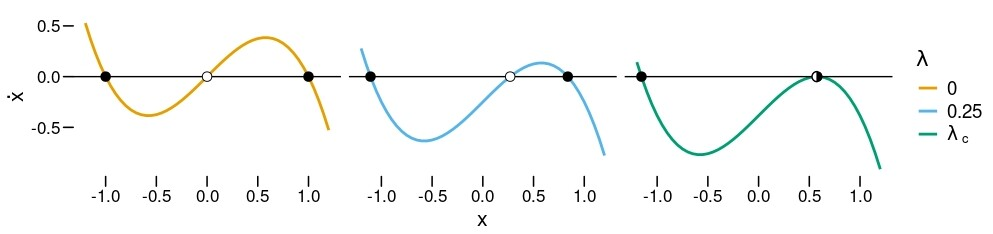
\includegraphics[scale = .5]{figures/double_well_plot.jpeg}
        \caption{The flow of the DW-potential dynamical system for varying values of $\lambda$.}
        \label{figure:DW_dynamic_plot}
    \end{center}
\end{figure}\\
By definition, the fixed points are the zeroes, which is typically marked as points in graphical representations. As a convention, stable fixed points are solid points, whereas unstable are hollow. Whether a specific fixed point is stable or unstable is easily deduced by simply looking at the flow of the graphs. When $\dot{x}_t$, i.e. $x_t'$, is below 0, the flow is to the left and vice versa; this simple reasoning allows us to understand the systems without doing any computations.

Now, notice the curious things happening for the value $\lambda = \lambda_c$. The system goes from having three fixed points: Two stable and one unstable, to just two fixed points: One stable and one half-stable. Mathematically, there is a real double root at the half-stable fixed point. Looking at the graph it is clear that this change in $\lambda$ results in a rather different qualitative behaviour of the system. From the definition of the double-well potential it is not difficult to see that increasing the value further would leave the system with just one stable fixed point. This is an entirely different overall behaviour compared to the other values of $\lambda$. This type of change in the characteristics of a dynamical system, we call a bifurcation. The specific value, $\lambda_c$, for which the changes occurs, we refer to as bifurcation points.\cite{Strogatz2019_gv} In applications, these points are also sometimes refered to as tipping points and the phenomenon as tipping.
To get an understanding of why this is occuring in this specific system, we compute the cubic discriminant. For a cubic polynomial in depressed form such as the dynamic (\ref{eq:originalDW}), this quantity is
\begin{align}
    \Delta_{\mathrm{DW}} = -\left(4(-1)^3+27\left(\lambda\right)^2\right) = -27\lambda^2 + 4. \label{eq:DW_discriminant}
\end{align} 
Whenever the result is positive; there are three solutions, when it is zero, there are two solutions. Finally, for negative values, there is only one solution to the cubic polynomial. The discriminant is a second degree polynomial in the parameter $\lambda$ and it has roots $\pm \frac{2}{3\sqrt{3}}$. The system depicted in figure \ref{figure:DW_dynamic_plot} uses the positive root as the value of $\lambda_c$. Yet, it is not difficult to imagine that decreasing the value of $\lambda$ would result in a mirrored, but completely analagous qualitative change to the one we observe in figure \ref{figure:DW_dynamic_plot}. Mathematically, this is due to $\Delta_{\mathrm{DW}}$ being positive for values of $\lambda$ between the two roots and negative outside. In the following, we focus on the positive root; though it should be noted that our reasoning is not limited to this bifurcation point. \\\\
$\lambda_c$ and the half-stable fixed point pertaining to it constitute an example of a specific type of bifurcations known as saddle-node bifurcations. For this value of $\lambda_c$ the stable fixed point is found at $x_1^* = -\frac{2}{\sqrt{3}}$, and the half-stable is $x_2^* = \frac{1}{\sqrt{3}}$. These are the solid- and partially solid points on the right graph in figure \ref{figure:DW_dynamic_plot}. We study the behaviour of the system close to the pair $(x, \lambda) = (x_2^*, \lambda_c)$ by a Taylor expansion of $f_{\mathrm{DW}}$ to the second order around the $x$-value and first order around the $\lambda$-value. This yields
\begin{align}
    f_{\mathrm{DW}}(x_t,\lambda)&\approx \frac{\partial}{\partial x_t}f_{\mathrm{DW}}(x_2^*,\lambda_c)(x-x_2^*) + \frac{1}{2}\frac{\partial^2}{\partial x_t^2}f_{\mathrm{DW}}(x_2^*,\lambda_c)(x_t-x_2^*)^2 \nonumber \\
     &+ \frac{\partial}{\partial \lambda}f_{\mathrm{DW}}(x_2^*,\lambda_c)(\lambda - \lambda_c) = -\sqrt{3}\left(x_t-x_2^*\right)^2 - \left(\lambda - \lambda_c\right) \nonumber \\&= -\left(\tilde{x}_t^2 + \tilde{\lambda}\right), \label{eq:prototypicalSaddleNode}
\end{align}
where $\tilde{x}_t = 3^{\frac{1}{4}}\left(x_t-x_2^*\right)$ and  $\tilde{\lambda} = \lambda - \lambda_c$. That is for values close to the bifurcation point the dynamic behaves similarly to that of this function, which is a quadratic polynomial in $x$ and linear in $\lambda$. Not only, is it a quadratic is $x$, it is also a rather simple quadratic with linear and intercept terms equal to zero. With $x_2^*$ being a fixed point, this was expected for the intercept. However, that the derivative of $f_{\mathrm{DW}}$ also evaluated to zero was not obvious. In fact, systems with bifurcations that locally around its bifurcation point behave in this manner are exactly what we understand by a system with saddle-node bifurcation. It is clear that any system with this type of Taylor-expansion around the bifucartion point will have a saddle-node bifurcation, as we can always scale and shift the dynamics to that of (\ref{eq:prototypicalSaddleNode}). For this reason, this particular form of dynamics is known as the prototypical- or normal form of the saddle-node bifurcation. Similar, calculations for the other bifurcation point of the double well model will leave us at the additive inverse of \ref{eq:prototypicalSaddleNode}. So in complete generality the normal form is
\begin{align}
    \mathrm{d}x_t = \pm\left(x_t^2 + \lambda\right)\mathrm{d}t
\end{align} 
As we see in the calculations of (\ref{eq:prototypicalSaddleNode}), these forms do not care about scaling and shifting, whence we write the normal form as
\begin{align}
    \mathrm{d}x_t = \pm\left(A\left(x_t - m\right)^2 + \lambda\right)\mathrm{d}t, \label{eq:standardform}
\end{align}
where $A>0$. Note that $x_t$ is not the same as the one from the double-well potential from earlier; we live with this ambiguity to avoid introducing too much notation.\\ In sum, we have illustrated that for some systems, which change qualitative behaviour at some parameter values; these systems behave roughly as what we refered to as the normal form of the saddle-node bifurcation, when $\lambda$ is close to the bifurcation point. Studying the system (\ref{eq:standardform}), we first note that is has quadratic discriminant $\Delta_{\mathrm{sf}} = -4A^2\lambda$. That is, we have two solutions to \ref{eq:standardform}, i.e. the system has two fixed points, whenever $\lambda<0$, one fixed point for $\lambda = 0$ and zero otherwise. When they exist, the fixed points are given by
\begin{align}
    \mu\left(\lambda\right) = m \pm \sqrt{-\frac{\lambda}{A}}. \label{eq:fixedPoint}
\end{align}
The fixed points are one stable- and one unstable fixed point, when $\lambda<0$; and one half-stable when $\lambda=0$. Which of the two is stable or unstable depends on the sign of the normal form \ref{eq:standardform}. Instead of illustrating the bifurcation qua the flow graph, we depict the phenomenon with a so-called bifurcation diagram\\
\begin{figure}[h]
\begin{center}
    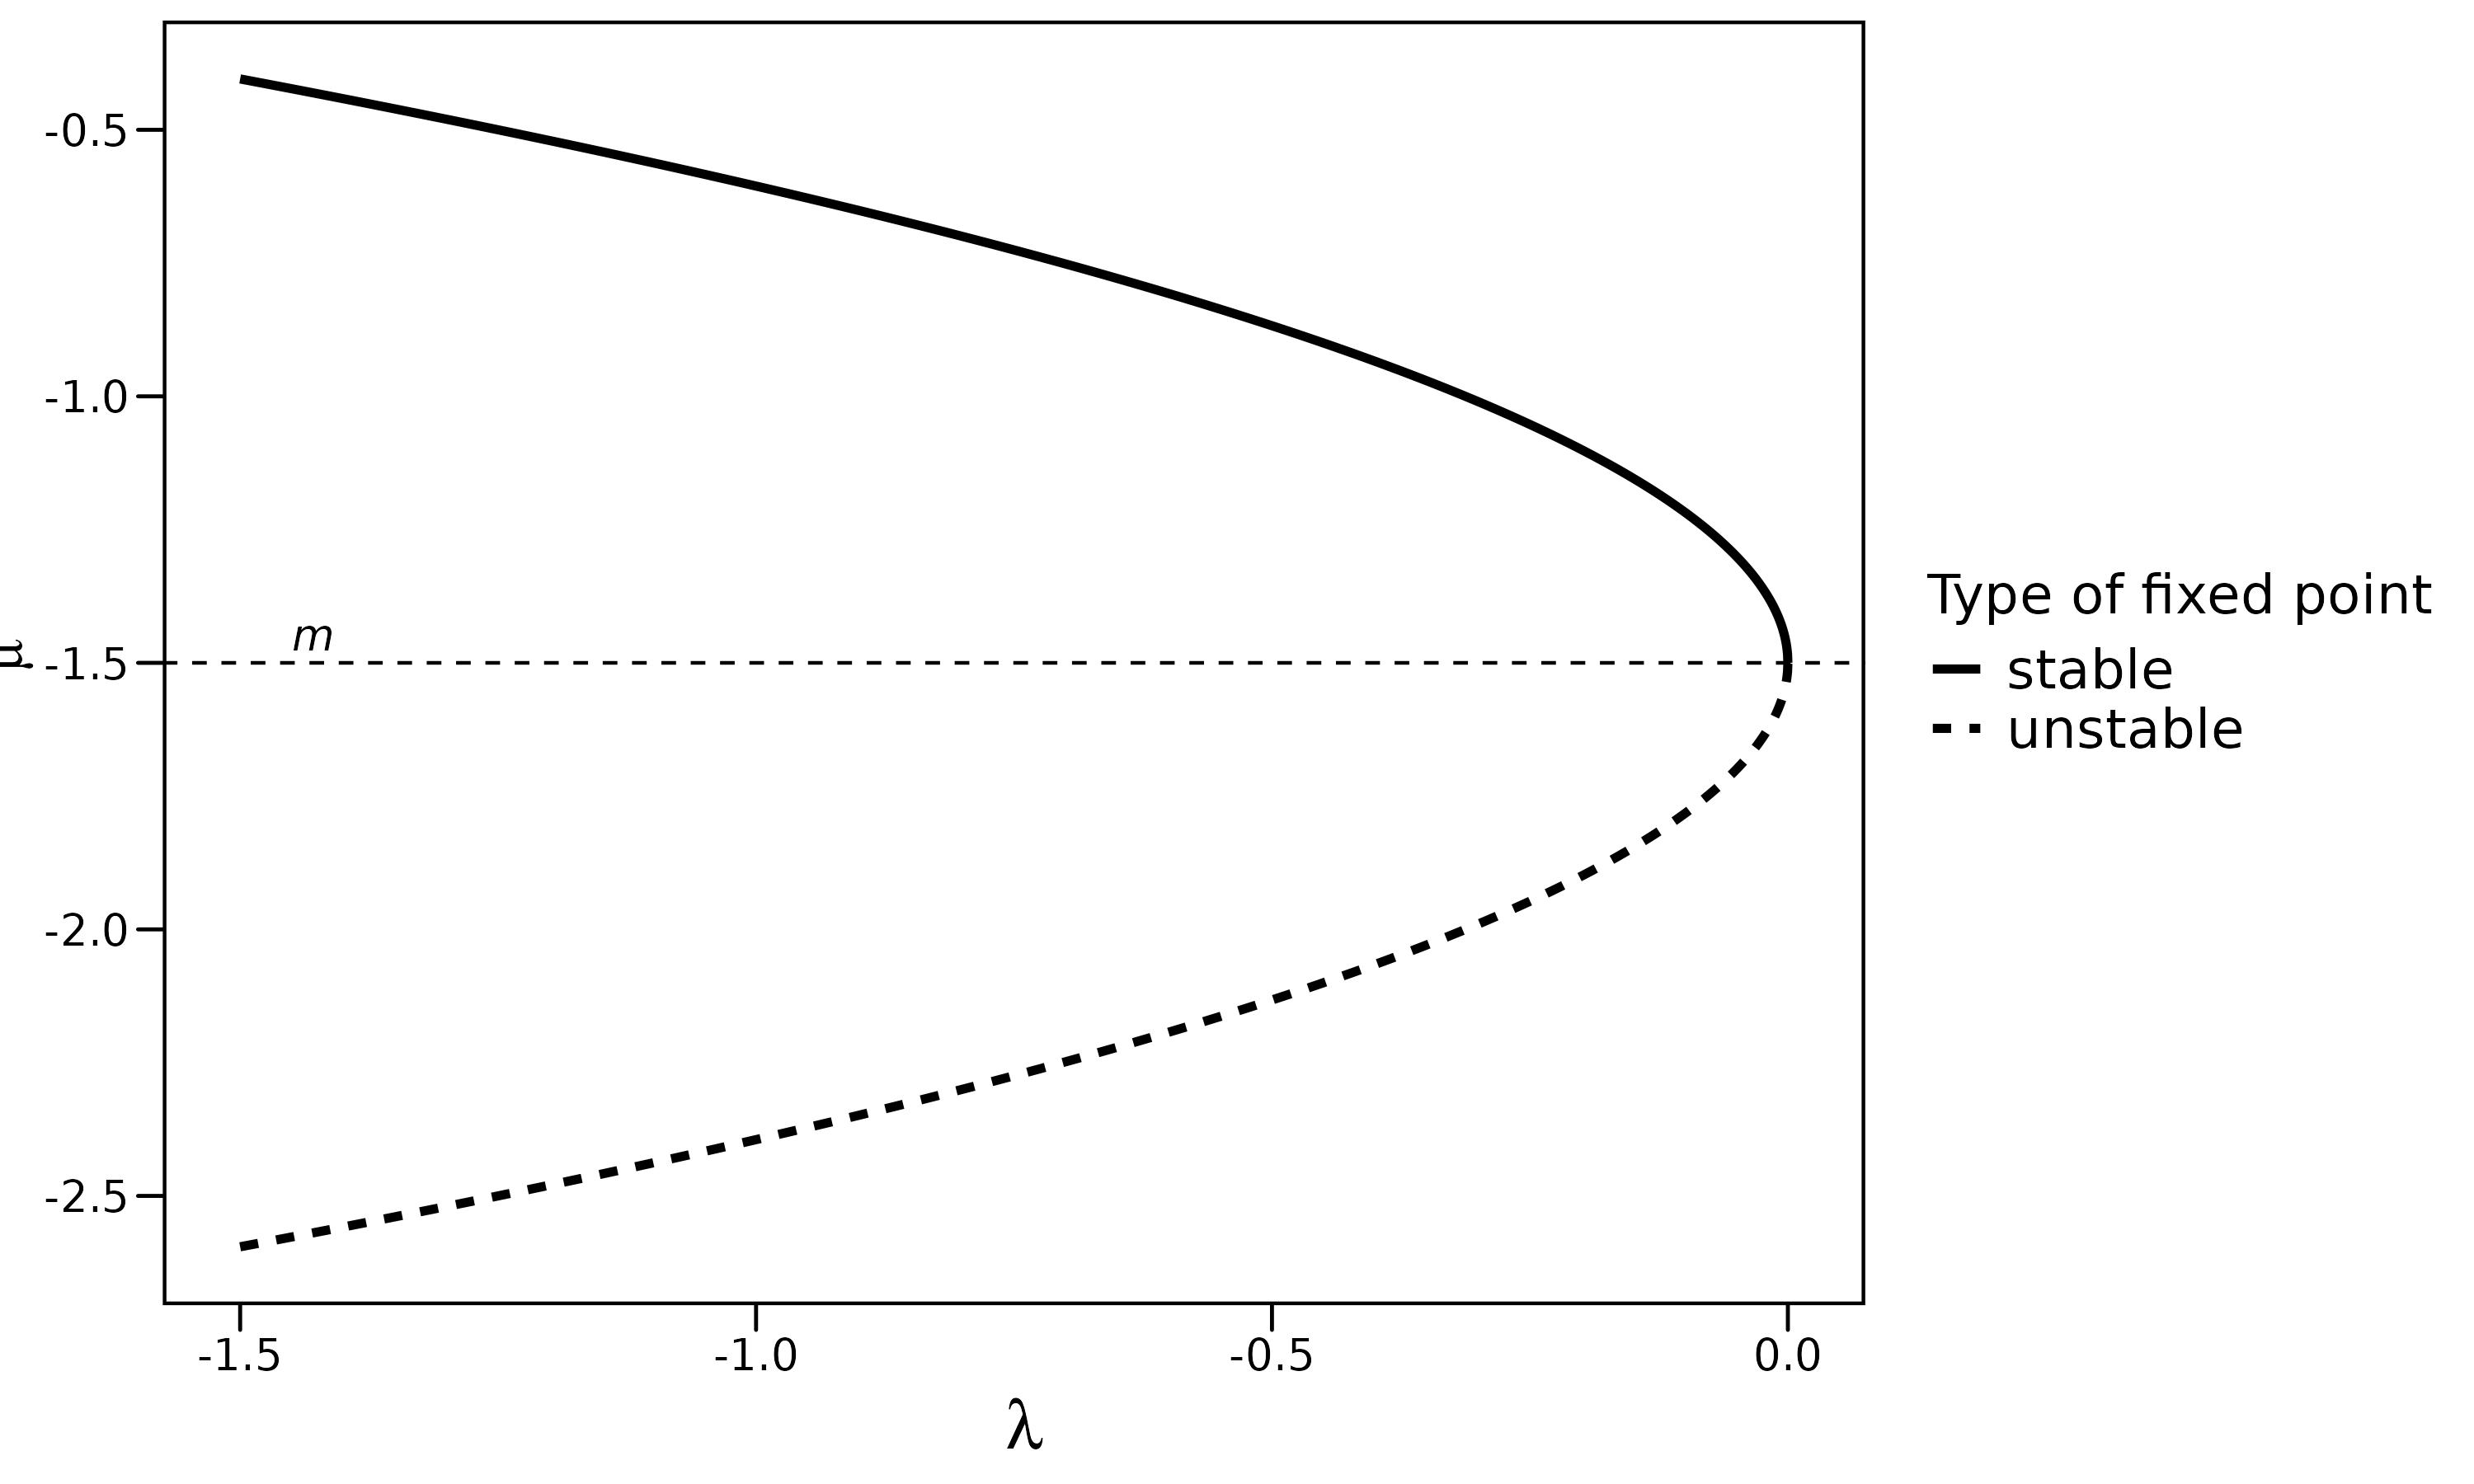
\includegraphics[scale = .4]{figures/bifurcation_diagram.jpeg}
    \caption{Bifurcation diagram of the scale and shifted normal saddle-node bifurcation.}
    \label{figure:bifurcationDiagram}
\end{center}
\end{figure}\\
Note that for $A$ and $m$ we picked $0.8$ and $-1.5$ respectively. The bifurcation diagram in figure \ref{figure:bifurcationDiagram} are the epitome of such diagrams for systems with a saddle-node bifurcation. As we have illustrated, any system with this type of bifurcation will locally for $\lambda \approx \lambda_c$ resemble (\ref{eq:standardform}) and hence their bifurcation diagram will too. One can also do the computations for the other branch of the normal form. In this case the fixed points in the bifurcation diagram are the same as before barring the fact that the types of the fixed points are swapped, i.e. for this system figure \ref{figure:bifurcationDiagram} would be mirrored around $m$.
\subsubsection{Tipping points}
We are now equipped with the necessary vocabulary to understand the model with which we estimate tipping points. We do not assume anything particular about the overall system dynamic other than that the system has a saddle-node bifurcation. Thus, we know that sufficiently close to the bifurcation point, we can consider the scaled and shifted prototypical saddle-node bifurcation system (\ref{eq:standardform}) in the general system's stead. For fixed $\lambda < 0$ in (\ref{eq:standardform}) the system is overall stable and converges to the stable fixed point, when we are not too far away from it. However, there are values, where the flow  diverges. Imagine that we are in the negative branch of (\ref{eq:standardform}); this is the situation depicted in figure \ref{figure:bifurcationDiagram}. As can be seen in the graph, the system diverges even when $\lambda<0$, if the process finds itself below the unstable fixed point. Furthermore, when $\lambda>0$ the system always diverges.

To estimate a tipping point with this model, is to estimate a point in time or the occurence of an event at which this abrupt change in characteristic of the system happens. Typically, this is done as a time point, which is also what we will do by modelling a ramping of $\lambda$ from some base value $\lambda_0$ it finds itself in, when the system is stable overall. We imagine that when we have observed the system for some time, $t_0$, it is disturbed or altered in some way that begins the ramping. There are several different ways this can be modelled, but here we let $\lambda$ depend on time, $t$, explicitly in the following way
\begin{align}
    \lambda_t = \lambda_0\left(1 - \max\left\{\frac{t - t_0}{\tau_c},0\right\}\right)^\nu, \label{eq:lambdaRampDefinition}
\end{align} 
which is the model from \cite[equation (2)]{Ditlevsen2023} with the addition of the parameter, $\nu>0$. As said $t_0$ can be understood as the time when ramping of $\lambda_t$ starts. The parameter $\tau_c$ is the amount of time after ramping begins for $\lambda_t$ to become zero. This is the point, when the two fixed points in \ref{figure:bifurcationDiagram} become one. That is, the point in time, where the dynamics of the system changes significantly: The tipping point. \\\\
Now, it is crucial to understand that the normal form is only a good approximation for a system with a saddle-node bifurcation close to its bifurcation point. Far from the tipping point or after the system has tipped the dynamics of the normal form are no longer a good approximation of the underlying dynamics. Put differently, our model does not allow us to infer anything about the system after it has tipped. Furthermore, we must observe the system sufficiently close to the bifurcation point for the dynamics to be close to the normal form. How close depends on the system at hand. These facts are, of course, significant downsides to the model. However, having such lean assumptions results in simple models: We can be completely agnostic about the actual dynamics of the system, because our main interest is the behaviour close to- or at the bifurcation point. As long as they have a saddle-node bifurcation, these dynamics could be arbitrarily complex and possibly difficult to infer anything about. Potentially, (\ref{eq:standardform}) is a huge simplification.
\subsubsection{Tipping in stochastic systems}
As is done in \cite[equation (1)]{Ditlevsen2023}, we introduce stochasticity into the normal form (\ref{eq:standardform}) to model the various uncertainties in the system. To reiterate from our introducing of stochastic differential equations, this results in a shift in the understanding of the solution, $X_t$. Now, for each point in time, $t$, the solution, $X_t$, to the noisy standard form has some distribution. While the original work assumed additive noise; we model the stochastic term as having the same noise as one of the Pearson diffusions (\ref{eq:pearsonDiffusion}). In sum, the model we consider is
\begin{align}
    \mathrm{d}X_t = \pm\left(A\left(X_t - m\right) + \lambda_t\right)\mathrm{d}t + \sigma\sqrt{\left(aX_t^2 + bX_t + c\right)}\mathrm{d}W_t, \label{eq:standardStochasticForm}
\end{align}
with $\lambda_t$ given by (\ref{eq:lambdaRampDefinition}). Note that the constants: $a, b$ and $c$ are picked such that the square-root is well-defined. In particular, we use the stochastic terms from the ergodic Pearson diffusions from table \ref{table:ergodicDiffusions}. To refer to a specific model, we have coined the following nomenclature: We refer to a model via the Pearson diffusion from which it gets its stochastic term. This could for instance be the \textit{$t$-diffusion based} model or even the \textit{$t$-distribution} model, albeit the last name might be a bit confusing or misleading it is quite natural to use. Alternatively, we might refer to the models by the way the noise enters, such as the model with \textit{linear} noise or the model with \textit{additive} noise. Although it might be obvious, it needs to be pointed out that a specific model inherits the state space of the pearson diffusion it shares stochastic term with in the way that the state space of models are always subspaces of the state space of the Pearson diffusion. The state spaces can be seen in table \ref{table:ergodicDiffusions}. Though, in this case the specific drift term in (\ref{eq:standardStochasticForm}) implies that the state space of a model correspond exactly to the state space of the Pearson diffusion it uses.\\\\
For clarity, $W_t$ is a brownian motion defined in (\ref{eq:brownianMotion1})-(\ref{eq:brownianMotion3}). This means that the solution to (\ref{eq:standardStochasticForm}) is an Ito process. Extending dynamical systems in this way is commonplace in various applied settings such as physics or finance. As said earlier, a way we typically motivate these kinds of constructions is, if we have a deterministic model for the well understood dynamics of the system. This could for instance be the drift term of (\ref{eq:standardStochasticForm}), which models the general behaviour of the system well: in this case that it has a saddle-node bifucartion. However, in the real world there might be elements that cannot be captured by the drift. Introducing a stochastic term into the dynamics lets us model the fact that there are parts of the system we do not understand or we do not want to model deterministically, because they are too complicated. Alternatively, we could use stochastic modelling, because our measurements are too inaccurate or noisy in some manner \newpage
\noindent With the scalar weak order 2.0 Ito-Taylor method described in section (\ref{subsubsec:Discretization}) we draw three sample paths with the same realizations of $W_t$ for each of the models to illustrate how they differ. In the graph one row corresponds to one path. The model we use is the one with a negative sign in front of the drift in (\ref{eq:standardStochasticForm})
\begin{figure}[h]
    \begin{center}
        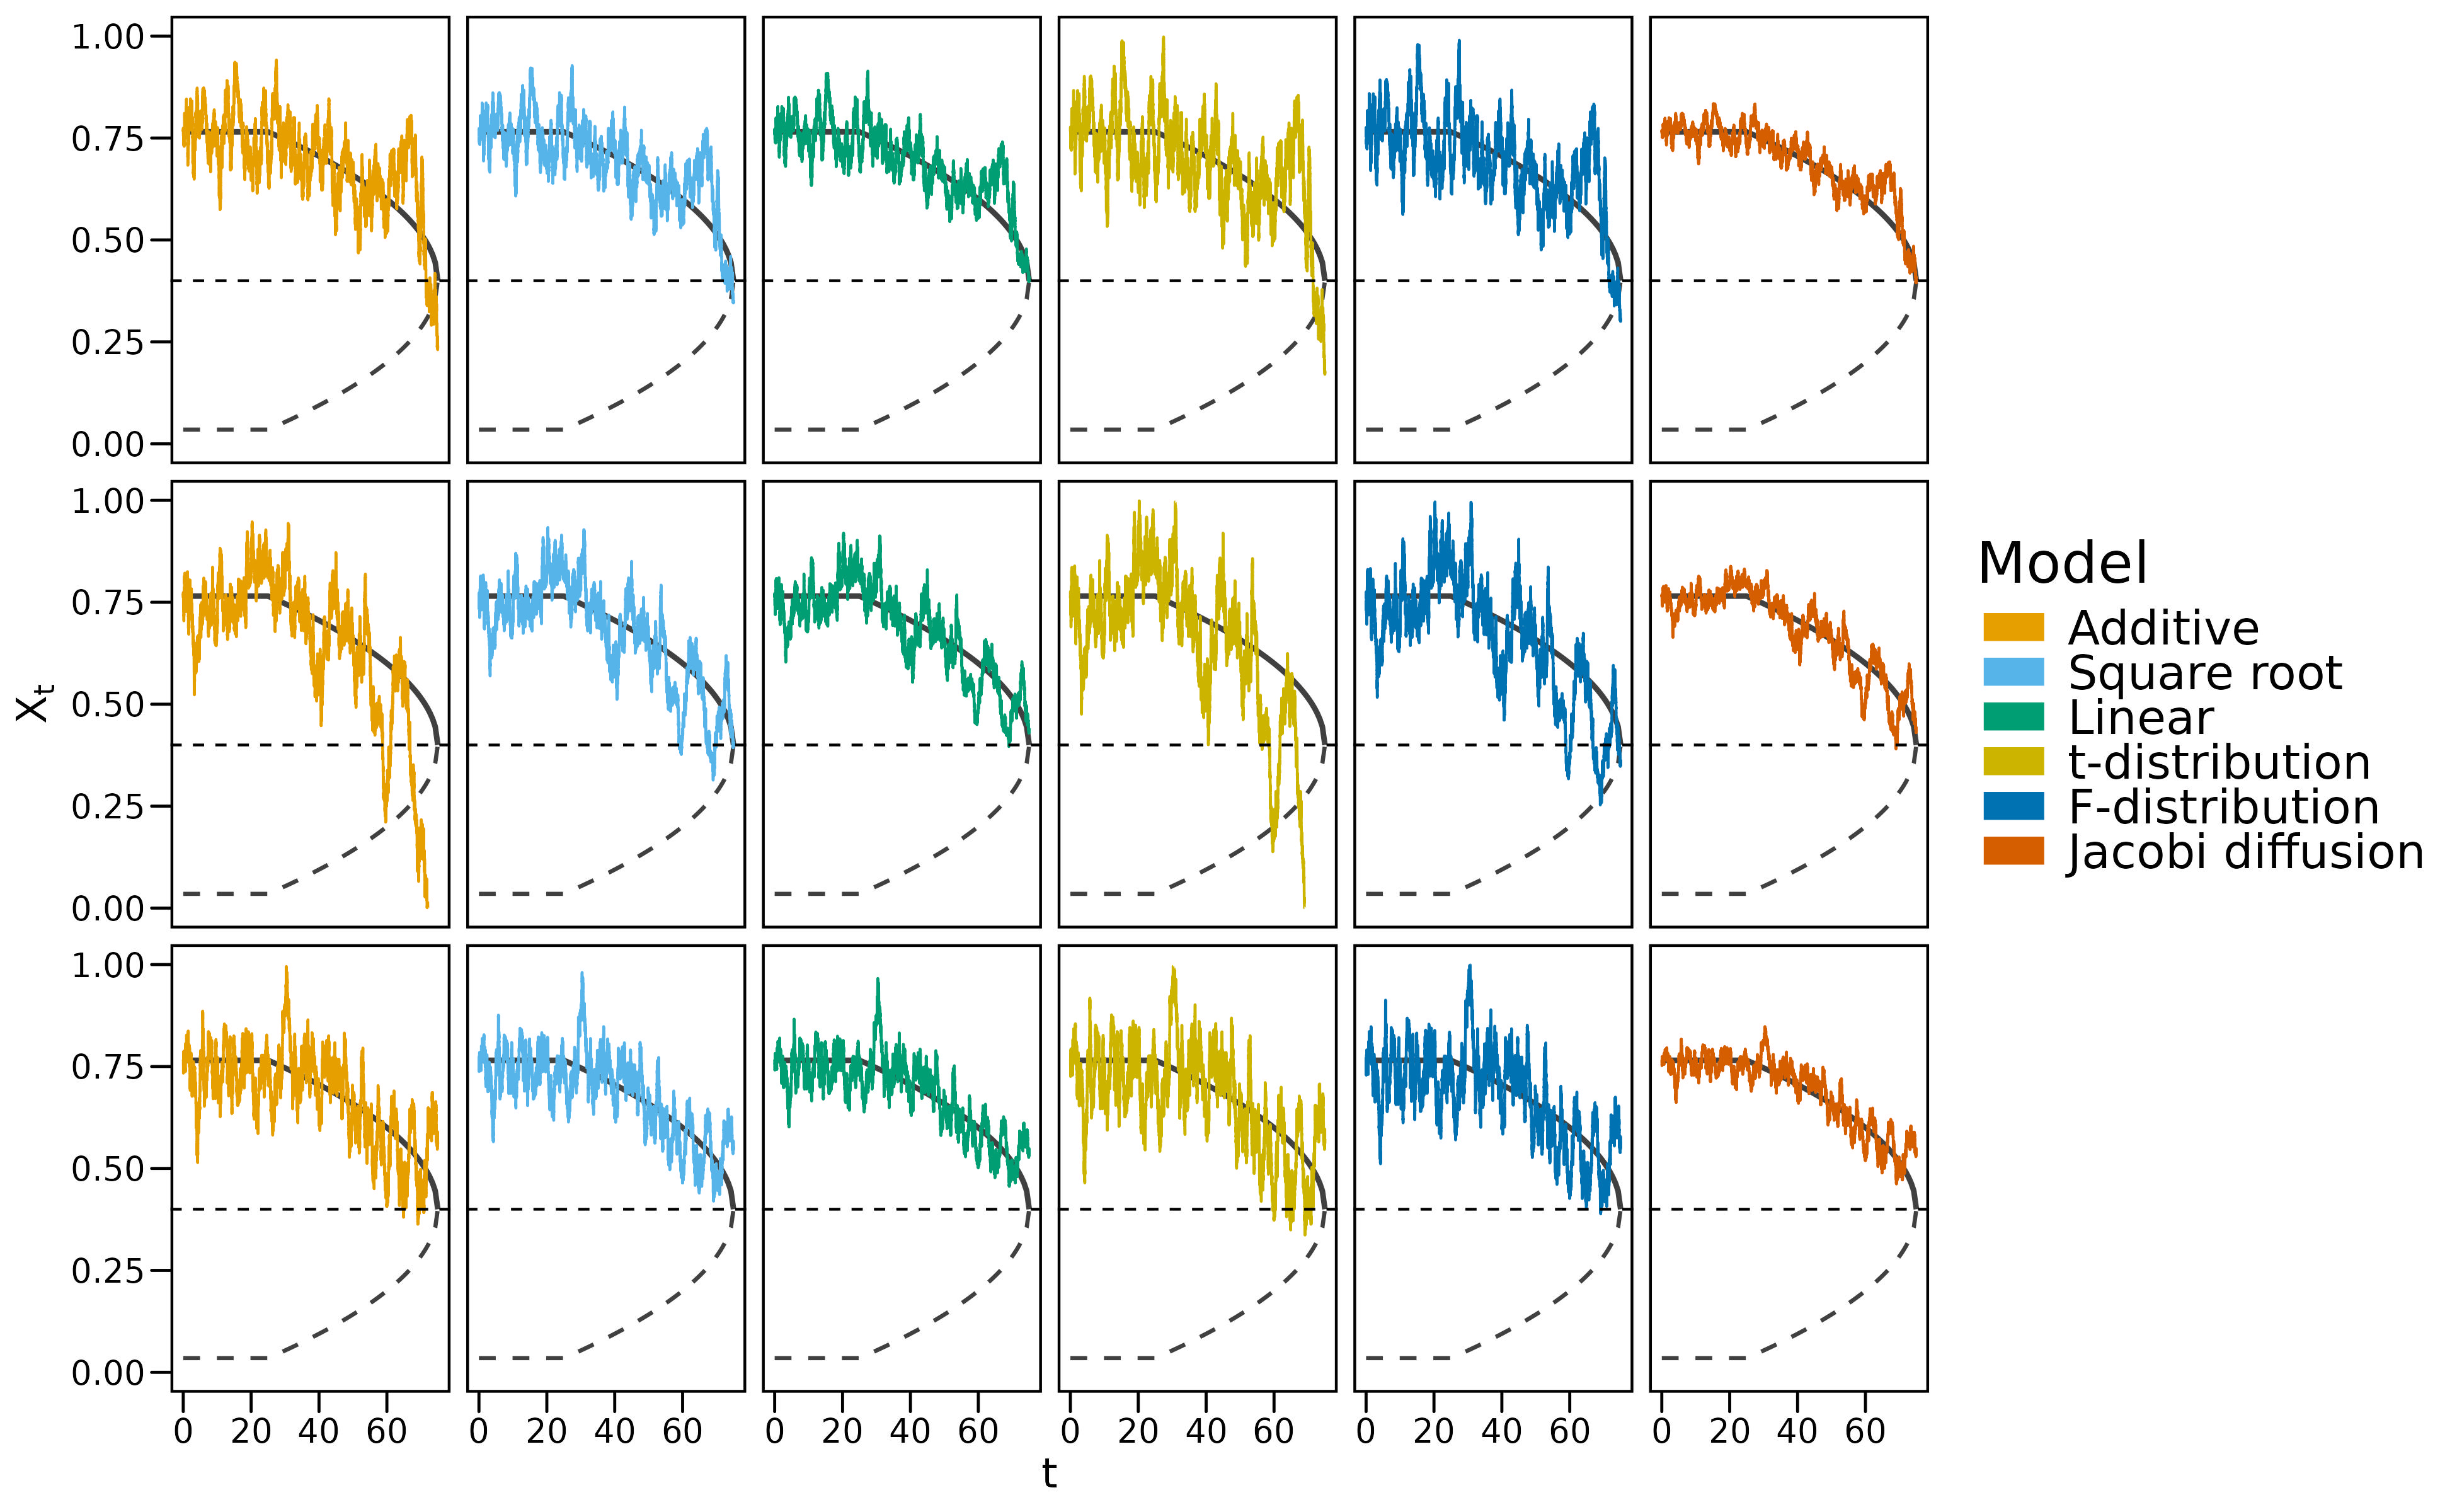
\includegraphics[scale = .1]{figures/sample_paths_plot_small_scale.jpeg}
        \caption{The dynamics of (\ref{eq:standardform}) with the six different noise terms from table (\ref{table:ergodicDiffusions}) applied to the same three realizations of a brownian motion.}
        \label{figure:samplesFromAllDifferentModels}
    \end{center}
\end{figure}\\
All the samples were drawn with parameters, $A = 1.5, m = 0.4, \lambda_0 = -0.2, \sigma = 0.1$ and $\nu = 1$. These parameters are carefully selected to ensure that we are in the state space of all processes in table \ref{table:ergodicDiffusions}. The process is started at time $0$ in its stable fixed point and starts ramping at $t_0 = 25$. The bifurcation point was set at time $75$, which means that $\tau_c = 50$. In sum, this means that in accordance with (\ref{eq:fixedPoint}) and (\ref{eq:lambdaRampDefinition}) the stable and unstable fixed points start moving from $m\pm\sqrt{\frac{\lambda_0}{A}}$ at time $t_0$ toward $m$ at time $t_0 + \tau_c$. Similarly to figure (\ref{figure:bifurcationDiagram}) this is depicted using a solid and dashed line respectively. The smaller horizontal dashed line they meet at is naturally, $m$. This is the effect of the specific form of ramping in (\ref{eq:lambdaRampDefinition}) when $\nu = 1$, i.e. a square-root evolution of the fixed points towards $m$ at the tipping point. This is exactly the effect of the ramping model from \cite{Ditlevsen2023}. Regardless of the noise, all the models have a bifurcation tipping at time $t_0+\tau_c$, the point we have simulated up to. However, due to the random nature of the brownian motion in the stochastic term not all models tip at that point. As we discussed with regards to figure \ref{figure:bifurcationDiagram}, the deterministic part of the process will diverge from below the unstable fixed point. We see that the additive noise model as well as the model with stochastic term from the ergodic diffusion with the $t$-distribution as its stationary distribution, cross the unstable fixed point prematurely twice. This phenomenon is called noise induced tipping and is exclusively a phenomenon in the study of dynamic system with stochasticity. All of the models are, in principle, always able to tip via noise. Still, for this to have any significant chance of happening the noise has to be on a scale that compares with the jump the process needs to make. In our case, this jump is the distance between the stable- and unstable fixed points at any given time point. However, the closer the path gets to the bifurcation point, the smaller the jump has to be. This is also why, we actually see the square-root- and linear noise based models as well as the $F$-diffusion model tip a bit before the bifurcation point in the first scenario. It should also be mentioned that a dynamic with a stochastic term does not have to have saddle-node bifurcation for it to be able to experience noise induced tipping.\\\\
Now, from table \ref{table:ergodicDiffusions} it is clear that the model with the same noise as the diffusion with the $t$-distribtion as its stationary distribution will always have diffusion term at least as large as the additive noise model. Thus, for the same realizations of $W_t$, if the model with additive experiences noise-induced tipping, it is quite likely that the $t$-diffusion based model will so too. The difference in the stochastic terms will be even more pronounced the further the values are from zero. This is also true for some of the other models. In figure \ref{figure:samplesFromAllDifferentModels} we have chosen parameters such that we are on the unit interval. This is to accomodate for the relatively confined state space of the Jacobi-diffusion based model. If we disregard this model, all the processes are well-defined on at least the positive reals. To illustrate what role the scale of our observations plays on the noise. We use first two Wiener realizations from earlier and depict the paths with the same $t_0, \tau_c, \sigma, A$, but to shift the scale away from the unit interval, we have picked $m = 3$ and $\lambda_0 = -1.75$. We get the following results
\begin{figure}[h]
    \begin{center}
        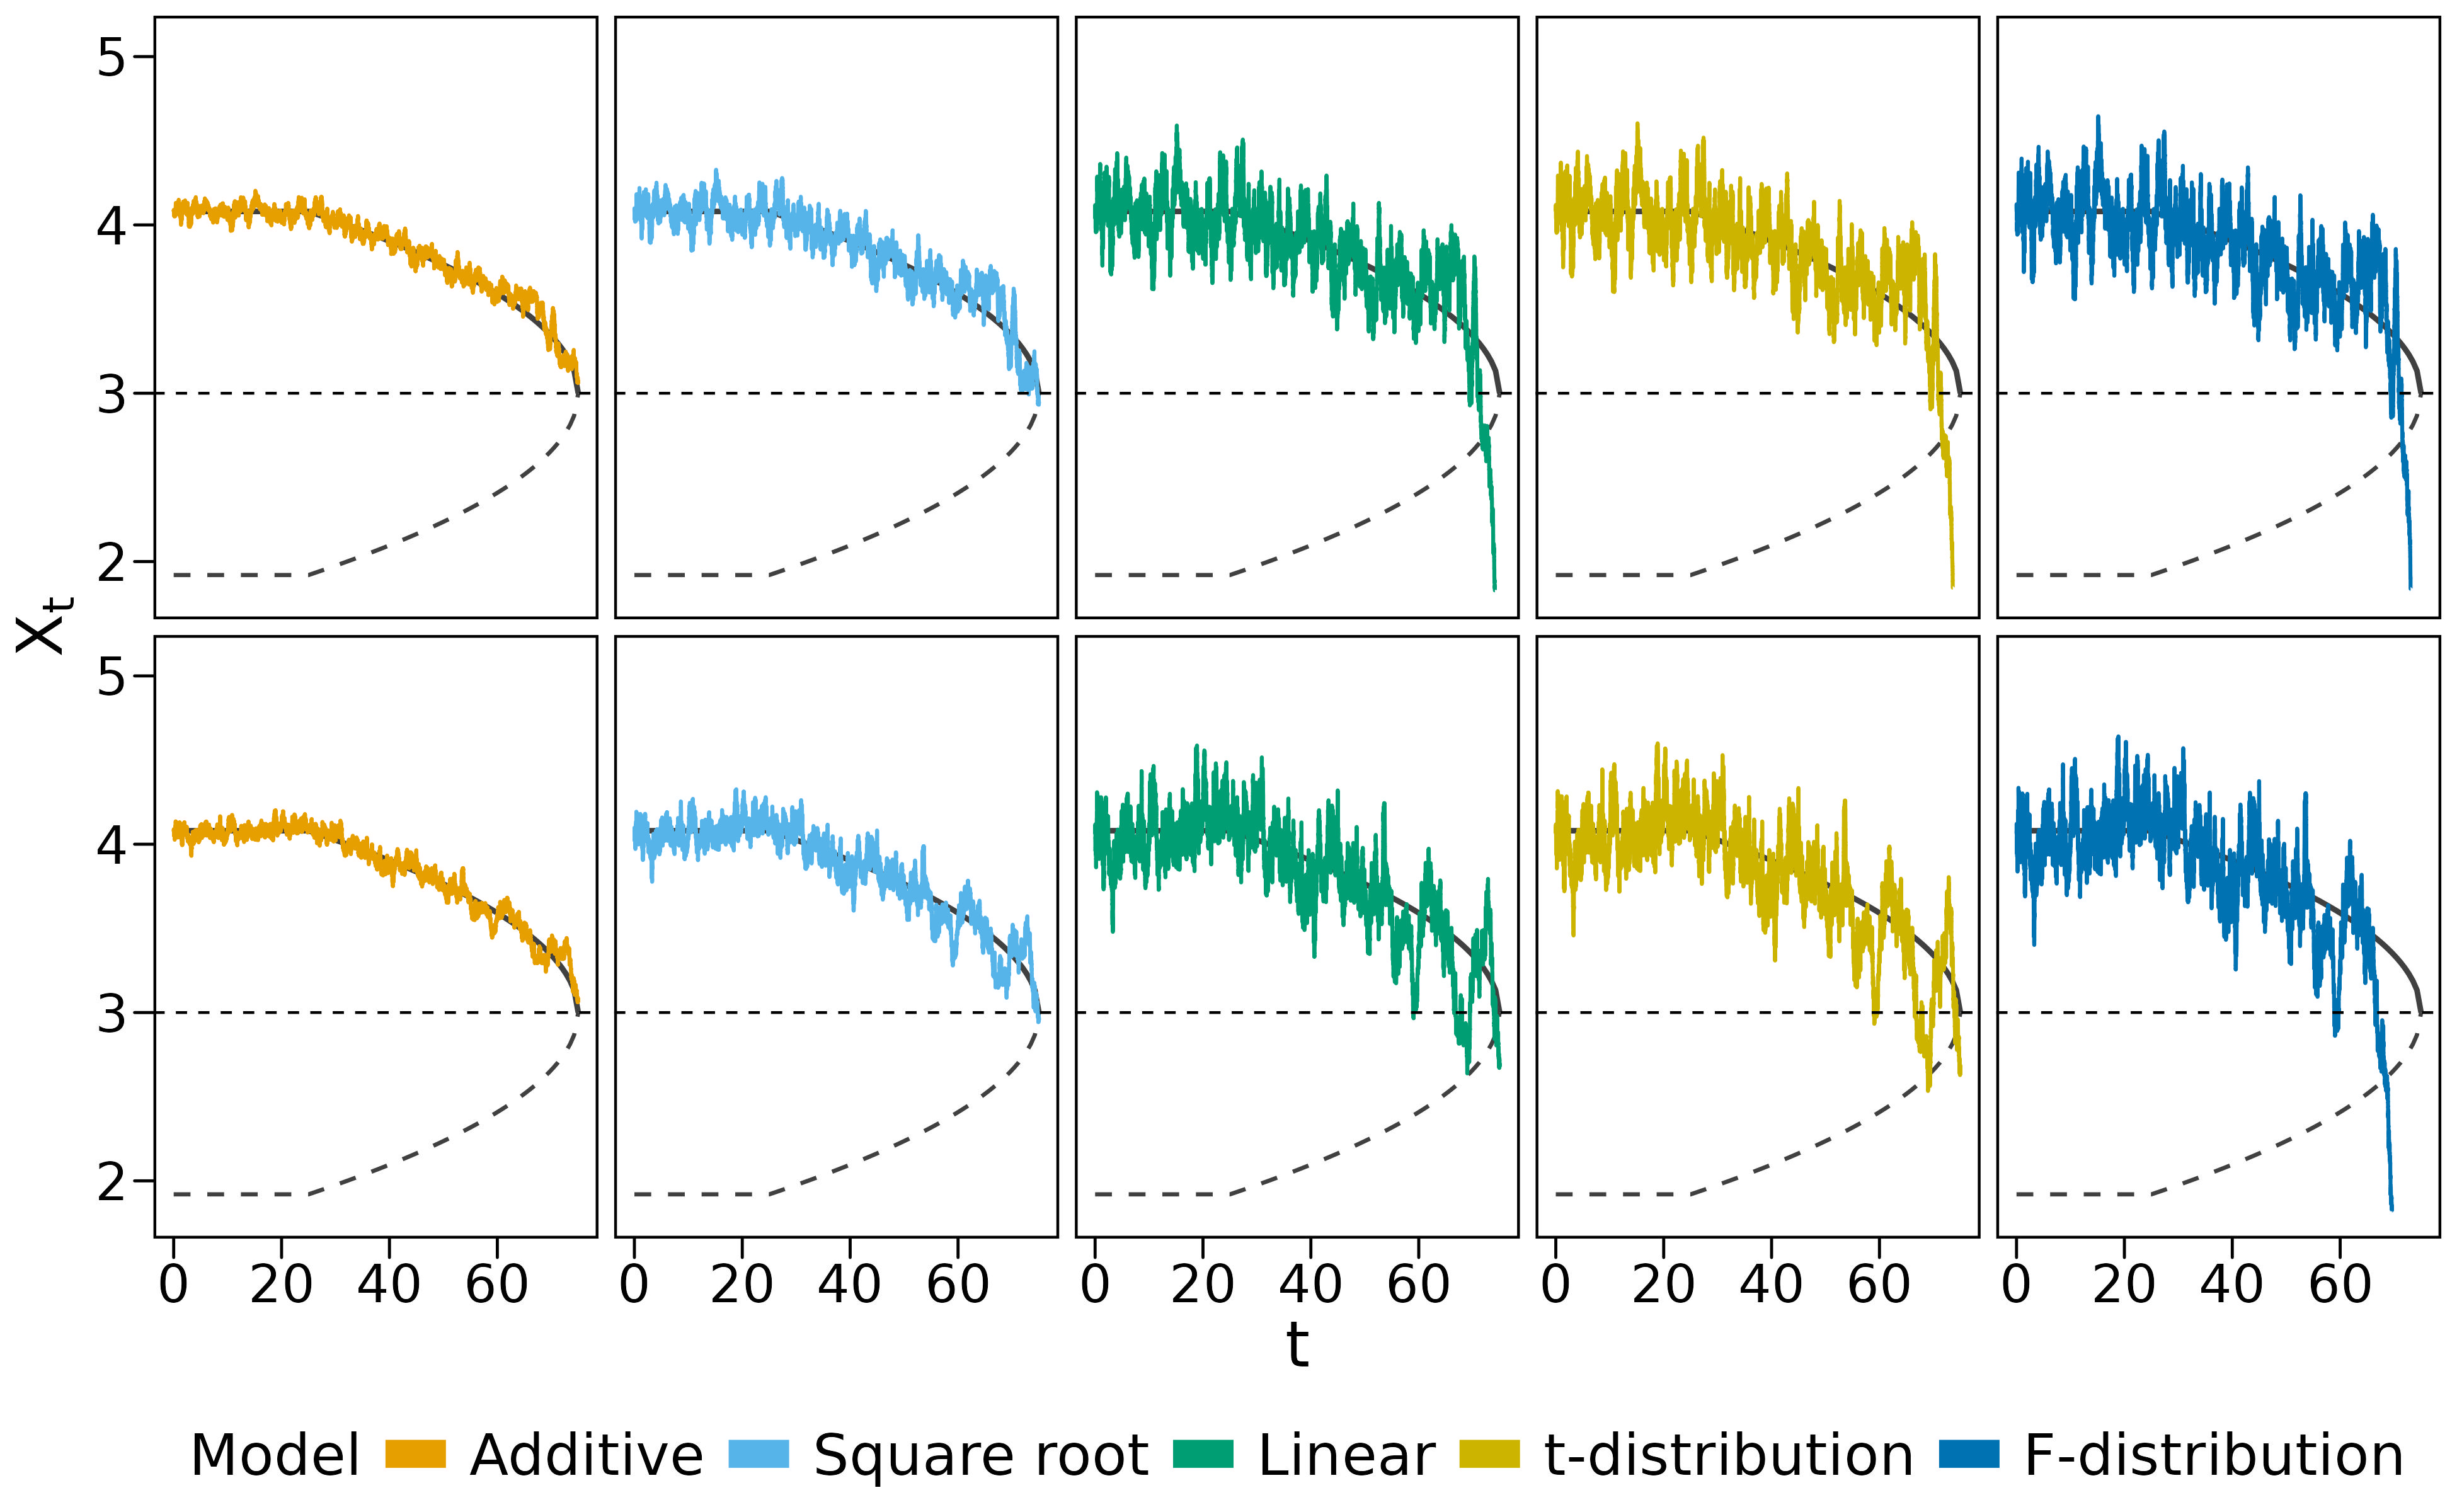
\includegraphics[scale = .1]{figures/sample_paths_plot_big_scale.jpeg}
        \caption{The dynamics of (\ref{eq:standardform}) shown on a different scale than figure \ref{figure:samplesFromAllDifferentModels} but with the same realizations of the Wiener process.}
        \label{figure:samplesFromFiveDifferentModels}
    \end{center}
\end{figure}\\
The overall impression of the respective models is quite different in figure \ref{figure:samplesFromFiveDifferentModels} than figure \ref{figure:samplesFromAllDifferentModels}. There is very little noise in the additive model in comparison to the other models with some kind of multiplicative noise. For instance the effect of the diffusion term in the $t$-diffusion based model is quite evident here. In addition, we observe how the $F$-diffusion based model along with the linear and square-root models undergo noise-induced tipping. Looking at the noise of the paths, it is clear what the difference in scale has meant for the qualitative feel of the square-root- and linear models. In figure \ref{figure:samplesFromAllDifferentModels} the square-root model was more noisy, while the opposite is the case in figure \ref{figure:samplesFromFiveDifferentModels}; here the linear model is more noisy. All this is not too surprising, when looking at the diffusion coefficients for the two processes. Neither is it surprising that the $F$-diffusion based model appear more noisy than both of them in both scales.\\\\
Lastly, we remark on the effect of the $\nu$-parameter, which is an extension of $\lambda_t$ \cite[equation (2)]{Ditlevsen2023}. As said this model corresponds to $\nu = 1$ as $\nu$ enters in an exponential manner into the bifucartion-parameter, which governs the fixed point of the drift according to \ref{eq:fixedPoint}. Apart from this fact the model works the same: $\lambda_t = \lambda_0$ for $t<t_0$, where ramping begins and $t=\tau_c + t_0$ is the tipping point. We use the same values of $m$ and $A$ as in figure \ref{figure:bifurcationDiagram} and pick $\lambda_0 = -2$, $\tau_c = 100$ and $t_0 = 10$, for the illustration of the fixed points as a function of time and $\nu$ in the model (\ref{eq:lambdaRampDefinition})
\begin{figure}[h!]
    \begin{center}
        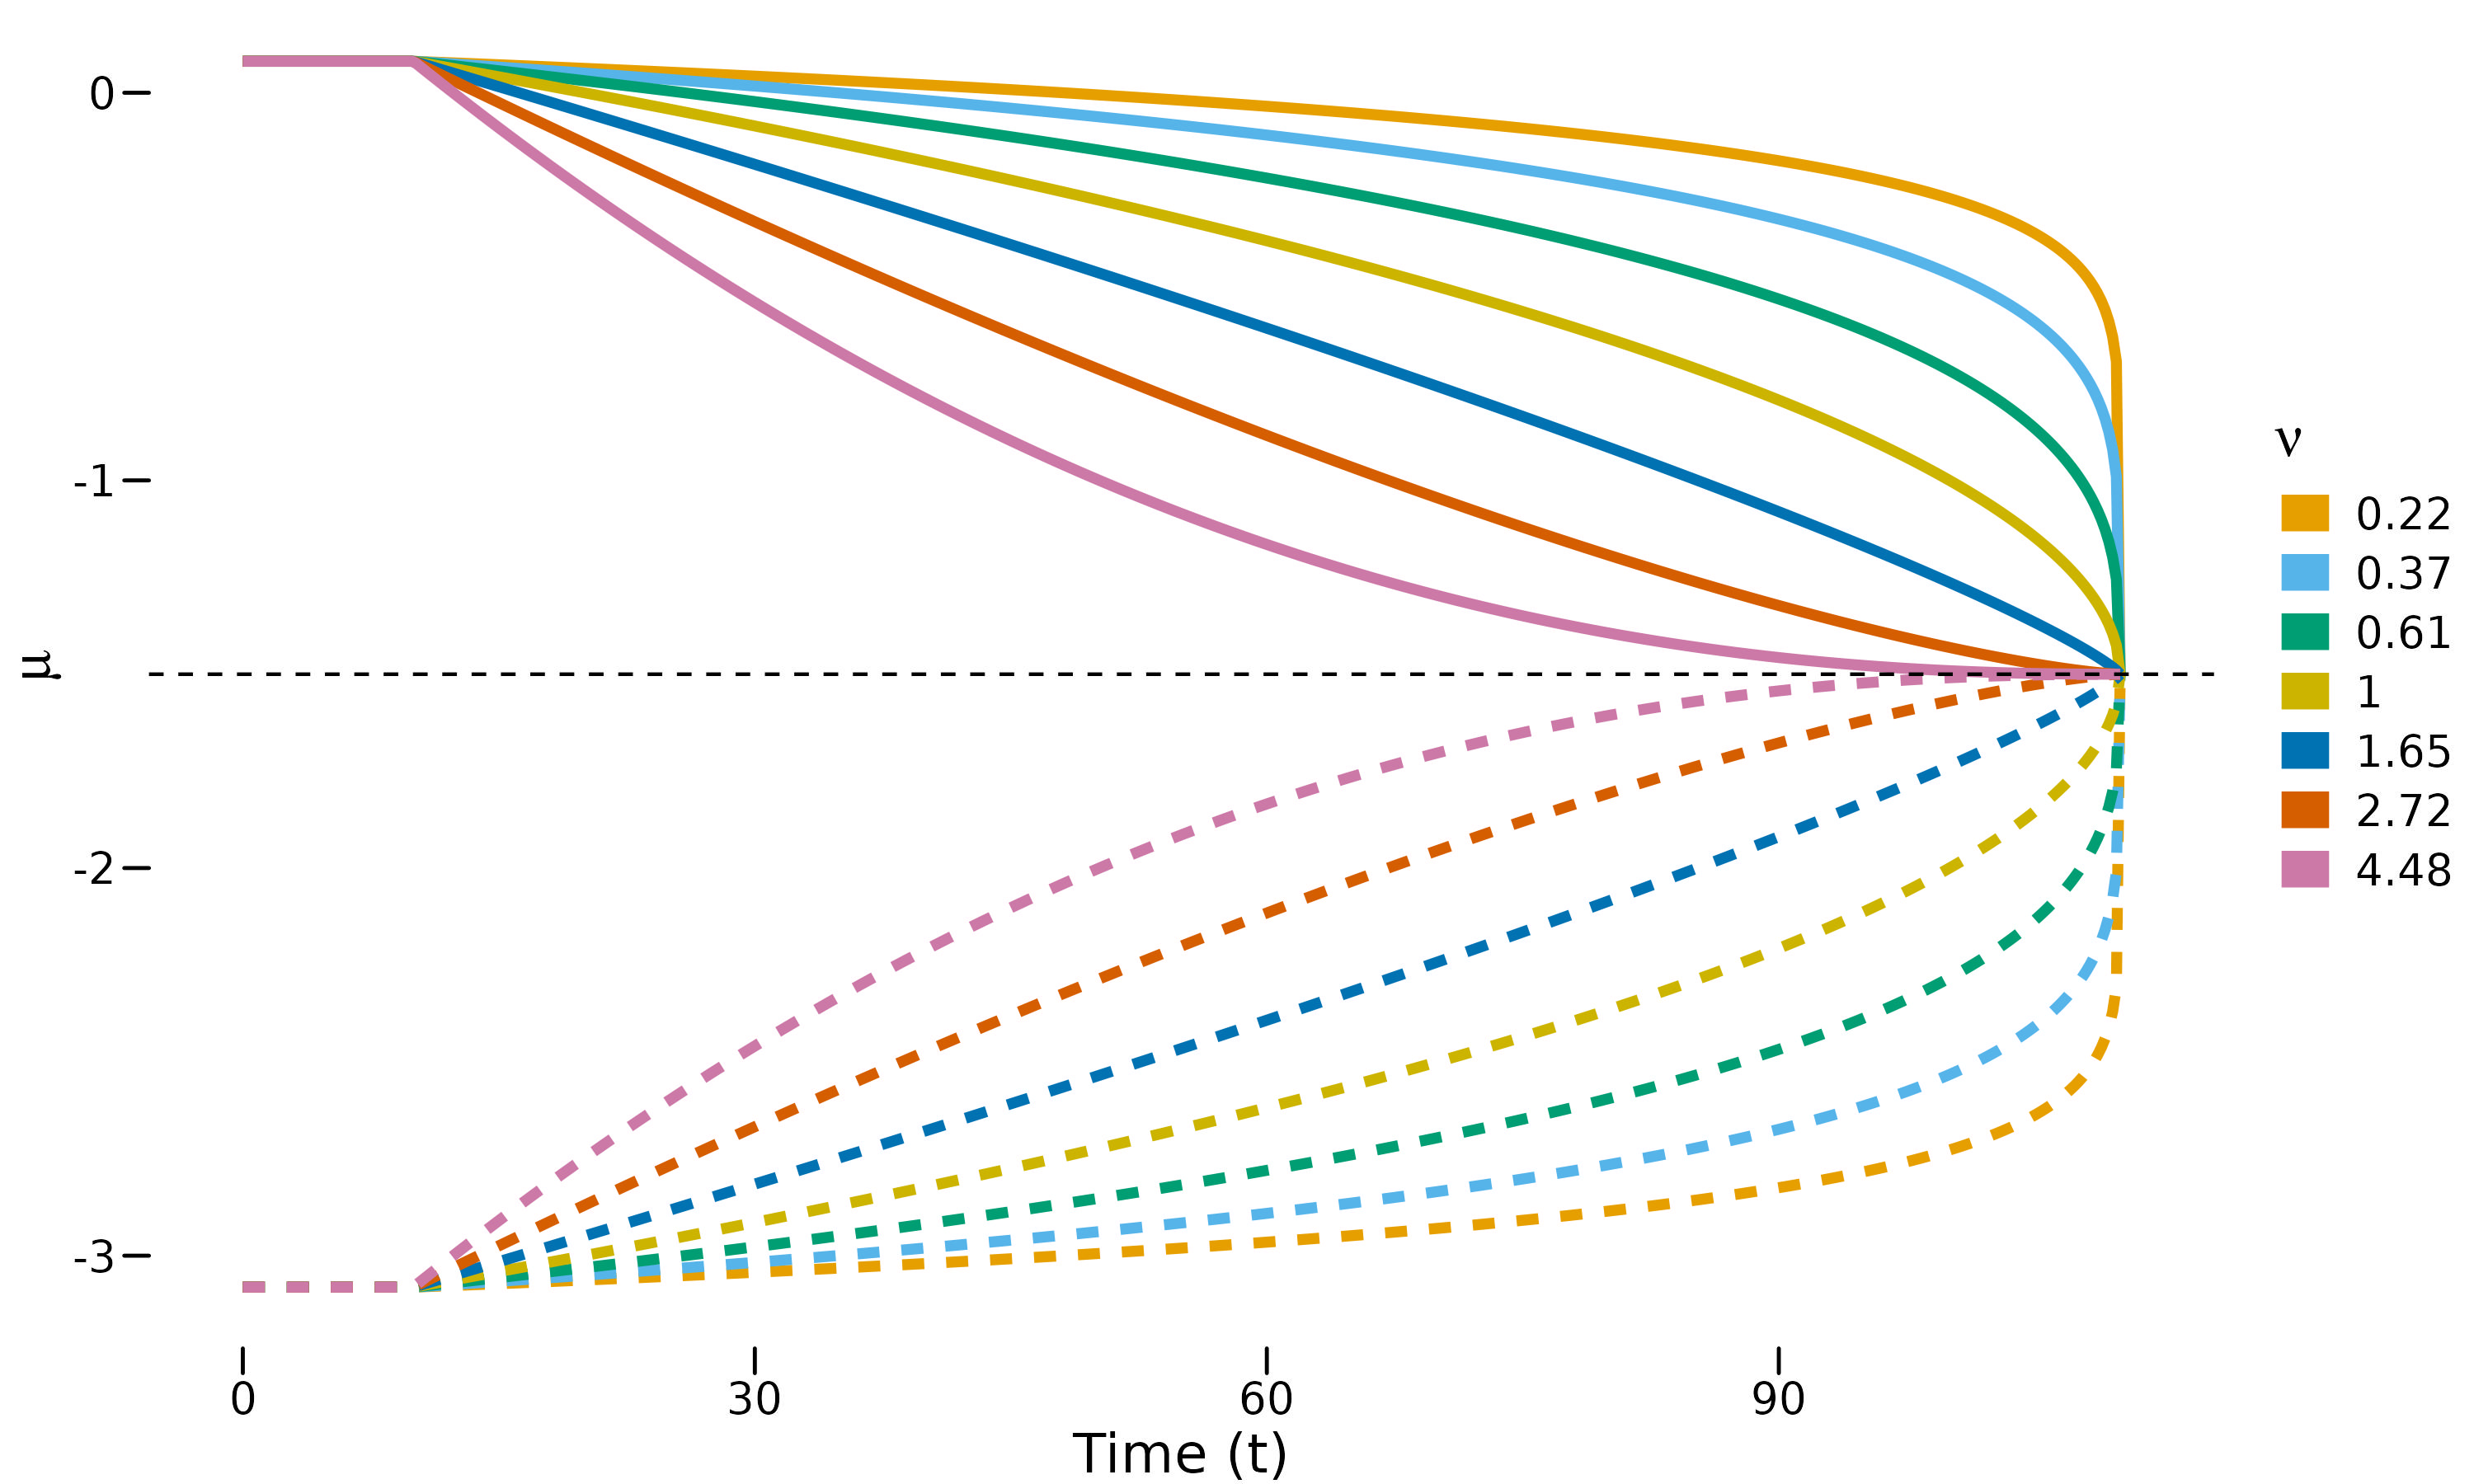
\includegraphics[scale = .1]{figures/nu_plot.jpeg}
        \caption{The fixed points of the prototypical saddle-node model with various $\nu$ in the ramping parameter}
        \label{figure:nu_plot}    
    \end{center}
\end{figure}\\
Again the fixed point at the bifucartion point, $m$, is marked by the horizontal dashed line. Looking at the graph we see that from the values of $\nu < 1$, we have to observe the process up to values fairly close to the bifurcation to actually see a significant change of $\lambda_t$ from $\lambda_0$. Conversely, for $\nu>1$ the two fixed points are closer together relatively early. During our later discussion, we comment more on the effect this can have on our inference; see for instance figure \ref{figure:mu_simulations_discussion_plot} for an example of how the different $\nu$ in figure \ref{figure:nu_plot} affect the sample paths. 

Still, there is a lot that can be said about the qualitative behaviour of these processes, we have just scratched the surface as of now. In any case, it is evident that the models are parametric. For us to do any inference on them, we need to be able to parameter estimation in stochastic differential equation. And this is something we have yet to introduce.
\subsection{Parametric inference for stochastic differential equations}
Here, we introduce the estimation methods that we use to do parameter estimation in stochastic differential equations. To be completely clear this means, that we wish to estimate $\theta\in\Theta\subseteq\mathbb{R}^p$. Often the entries in $\theta$ that parameterizes the two parts of the SDE will be different. In these cases, it is natural to split the parameter vector into the parts having to do with each term. For simplicity, we only have one parameter in the stochastic term, $\sigma>0$ and the process is autonomous. This mean we can write
\begin{align}
    \mathrm{d}X_t = b(X_t; \theta)\mathrm{d}t + \sigma\left(X_t\right)\mathrm{d}W_t, \label{eq:SDEInference}
\end{align}
We assume that we have samples $\mathbf{x} = x_{t_1},\dots x_{t_N}$ with some known temporal resolution, $\Delta t_k$, from the process (\ref{eq:SDEInference}); we do inference about the parameters by leveraging the markov property of Ito processes. This means that in order to do estimation, it is suffices to use the transition density - or approximations thereof. Though, as we discussed earlier, getting the transtion density involves solving the Kolmogorov forward equation (\ref{eq:fokkerPlanck}), which for the most part is not possible. Instead, we employ some approximation methods.

Traditionally the approximation is made using on the Euler-maruyama scheme, which we discussed in section \ref{subsubsec:Discretization}; the transition density based on this approximation is the euler-maruyama based estimator. However, in this thesis we only used the Euler-maruyama estimator in the initial development. The estimator is fairly easy to derive, implement and it is computationally quite efficient. Yet, it is quite biased even for moderately large stepsizes and notably so in very non-linear models \cite{SplittingSchemes}. In short, the method serves well as proof-of-concept or for testing purposes, but has limited use outside of this. As the estimator itself is ubiquitous in the litterature and does not play any part in actual inference, we do not introduce it here. Instead, we consider two other means of estimation. The Strang based pseudo-likelihood \cite{SplittingSchemes} and so-called approximately optimal martingale estimation equations \cite{StatisticalMethodsForSDE}.
\subsubsection{The Strang likelihood}
The Strang (S) based estimator is a method based on splitting schemes, which is a method stemming from the study of ordinary differential equations. With splitting schemes it is also possible to construct the Lie-Trotter (LT) based estimator. The common objective of the two methods is to approximate the transition density by splitting the stochastic differential equation into two parts that can be solved and then use the solutions to those in composition to construct an approximation for the transition density.

This strategy originates in the study of ordinary differential equations. When using it for stochastic differential equations it is important to construct the splitting such that the first part of it constitutes an SDE that in some way is sufficiently simple such that we can solve it, whereas the other part needs to be completely deterministic. That is, we assume that we are able to solve these systems by themselves, and that this gives us two seperate flows, $\varphi_{\Delta t}^{[1]}$ and $\varphi_{\Delta t}^{[2]}$: The solution to the simple SDE and the ODE, respectively, with some given stepsize, $\Delta t$. And in some composition, the two seperate flow should then, hopefully, be a good approximation of the actual flow that we cannot solve directly.

The difference between the Strang and the Lie-Trotter approximations is then the way in which the solutions are composed to give the approximation of the original system. They are composed in the following ways
\begin{figure}[h!]
    \begin{center}
    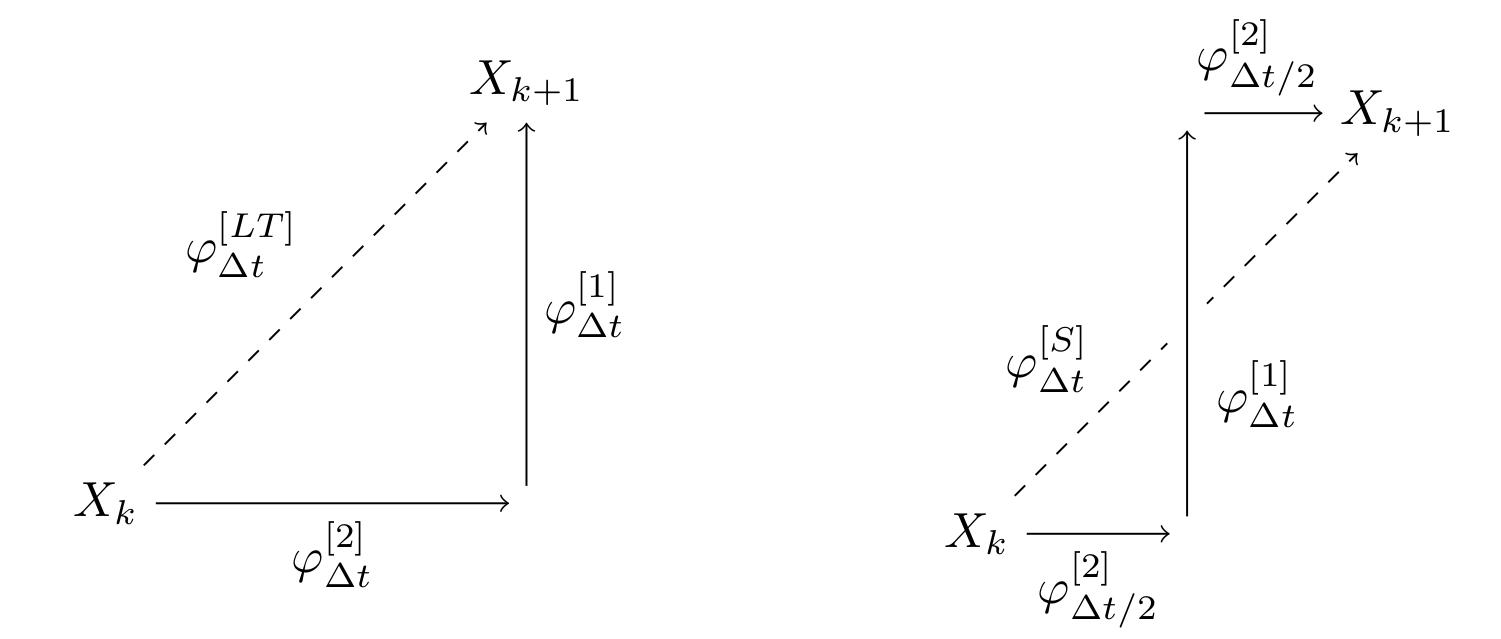
\includegraphics[scale = .185]{figures/strangAndLieTrotter.jpeg}
    \end{center}
    \caption{A diagram of the Lie-trotter- (left) and Strang (right) compositions}
    \label{figure:StrangAndLieTrotterPlot}
\end{figure}\\
Although they are quite similar overall, the one-step predictions of the transition densities given by the Strang splitting scheme is proven to be superior to that of LT; compare \cite[Proposition 3.4 and 3.6]{SplittingSchemes}. For this reason, we only consider the Strang splitting scheme but our ideas could very easily be adapted to Lie-trotter schemes. We start by looking at the Strang splitting on a general one-dimensional SDE with additive noise. Later we comment on the possible ways to use this method even for models with multiplicative noise.\\
\textbf{Models with additive noise}\\
General one-dimensional autonomous stochastic differential equations with additive noise can be written as
\begin{align}
    \mathrm{d}X_t = b(X_t; \theta)\mathrm{d}t + \sigma\mathrm{d}W_t, \label{eq:generalAdditiveNoiseSDE}
\end{align}
note that we have highlighted the dependence of some parameter, $\theta\in\Theta\subseteq\mathbb{R}^p$ in the drift. When we have additive noise, splitting schemes work by decomposing the process into a linear SDE and a non-linear ODE in the following way
\begin{align}
    \mathrm{d}X_t^{(1)} &= -\beta(\theta)\left(X_t^{(1)} - \mu(\theta)\right)\mathrm{d}t + \sigma \mathrm{d}W_t, &&X_t^{(1)} = x_0, \label{SDE_split}\\
    \mathrm{d}X_t^{(2)} &= N\left(X_t^{(2)}; \theta\right)\mathrm{d}t, &&X_t^{(2)} = x_0, \label{ODE_Split}
\end{align}
where the splitting is constructed such that the sum of (\ref{SDE_split}) and (\ref{ODE_Split}) is equal to (\ref{eq:generalAdditiveNoiseSDE}), meaning that $N$ is some non-linear defined as the difference between the drift in (\ref{eq:generalAdditiveNoiseSDE}) and (\ref{SDE_split}). Evidently, this splitting is not unique, and thus the way we construct the estimator will not be either. However, it turns out that any splitting of (\ref{eq:generalAdditiveNoiseSDE}) done in this way yields approximations of the transition densities that are equivalent asymptotically \cite{{SplittingSchemes}}. Yet, our choice might have an impact on the quality for finite samples. Additionally, in practice it is not difficult to imagine that some splittings are numerically more well-behaved than others. So we still have to carefully consider our splitting choice. The one we use for the most part is the heuristic provided in \cite[section 2.3 and 2.5]{SplittingSchemes}. The strategy presented here is: Construct (\ref{SDE_split}) as the linearization around the fixed points of the drift. This means, we use $b(X_t, \theta)$ from (\ref{eq:generalAdditiveNoiseSDE}) and solve the following equation
\begin{align}
     b(X_t; \theta) = 0,
\end{align}
in terms of $X_t$. Then set $\mu\left(\theta\right)$ to be equal to this solution and plug the value into the derivative of $b(X_t, \theta)$ w.r.t. $x$
\begin{align}
    \beta\left(\theta\right) = \left.\frac{\partial b(x; \theta)}{\partial x}\right|_{x = \mu\left(\theta\right)}.
\end{align}
The two components is used together to construct (\ref{SDE_split}).
Hereafter, (\ref{ODE_Split}) is calculated as the residual of the \ref{eq:generalAdditiveNoiseSDE} and our (\ref{SDE_split}). 

Recall that in the one dimensional case, the solution with stepsize, $\Delta t$, to the linear SDE is given by the flow
\begin{align}
    \varphi_{\Delta t}^{(1)}(x) = \exp\left(-\beta\left(\theta\right) \Delta t\right)\left(x - \mu\left(\theta\right)\right) + \mu\left(\theta\right) + \xi_{\Delta t}, \label{varphiTheoretical}
\end{align}
with $\xi_{\Delta t}\sim\mathcal{N}\left(0, \Omega_{\Delta t}\right)$. That is, the flow is gaussian with mean and variance
\begin{align}
    \mu_{\Delta t}(x; \theta) &= \exp\left(-\beta\left(\theta\right) \Delta t\right)\left(x - \mu\left(\theta\right)\right) + \mu\left(\theta\right) \label{linearSDEMean}\\
    \Omega_{\Delta t} &= \frac{\sigma^2}{2\beta}\left(1 - \exp\left(-2\beta\left(\theta\right)\Delta t\right)\right), \label{linearSDEVariance}
\end{align}
which we calculated in (\ref{eq:OU_solution}). For our purposes the solution to (\ref{ODE_Split}) exists and is unique; this is ensured by the Picard-Lindelöf theorem \cite[section 2.7]{Srkk2019}, since (\ref{ODE_Split}) is ordinary differential equations that in our case will be sufficiently regular for the assumptions from the theorem to hold. Still, we might find ourselves in a situation, where we cannot get a closed form solution to (\ref{ODE_Split}), simply due to the complexity of the ODE. In those cases, we use the Fourth Order Runge-Kutta method to solve it numerically \cite[p.541 equation (8)]{numericalAnalysis}.  
Nevertheless, we denote the solution with stepsize, $\Delta t$, $\varphi_{\Delta t}^{(2)}$. By figure \ref{figure:StrangAndLieTrotterPlot} the Strang splitting scheme then gives the approximation of the transition density as 
\begin{align}
    X_{t_{i+1}}^{(S)} = \varphi_{\Delta t / 2}^{(2)}\left(\mu_{\Delta t}\left(\varphi_{\Delta t/2}^{(2)}\left(X_{t_{i}}^{(S)}\right); \theta\right) + \xi_{\Delta t} \; ; \theta \right). \label{eq:classicStrangSplitting}
\end{align}
Due to the fact that (\ref{varphiTheoretical}) is gaussian, (\ref{eq:classicStrangSplitting}) is a non-linear transformation of a gaussian variable with the specified mean and variance. So by the density transformation theorem, this flow has the following negative pseudo-loglikelihood 
\begin{align}
    l^{[S]}(\mathbf{x}; \theta) &= -\sum_{i = 0}^{N - 1}\log\left(g\left(\left(\varphi_{\Delta t / 2}^{(2)}\right)^{-1}\left(x_{t_{i+1}}\right); \mu_{\Delta t}\left(\varphi_{\Delta t/2}^{(2)}\left(x_{t_{i}}\right); \theta \right), \Omega_{\Delta t} \right) \right) \nonumber \\
    &- \sum_{i = 0}^{N - 1}\log\left(\frac{\partial}{\partial x}\left(\varphi_{\Delta t / 2}^{(2)}\right)^{-1}\left(x_{t_{i + 1}}\right) \right), \label{eq:Strang_likelihood}
\end{align}
where $t_N$ is the index of the most recent sample in the data. (\ref{eq:Strang_likelihood}) is the Strang based pseudo-likelihood, and we say that the $\theta$ that minimizes this function is the Strang-based estimator. In (\ref{eq:Strang_likelihood}) $g$ is the gaussian density function with the specified mean and variance. 
To get the inverse of the solution to the ODE, we use the property $\left(\varphi_{\Delta t}^{(2)}\right)^{-1} = \left(\varphi_{-\Delta t}^{(2)}\right)$ \cite[Remark below equation (9)]{SplittingSchemes}, and solve the resulting ODE analytically or with the fourth-order Runge-Kutta. Finally, to get the derivative we use direct computation when possible and Richardson extrapolation, if we used the Runge-Kutta method before. For a differentiable function, $f$, a simple Richardson extrapolation approximates the derivative as
\begin{align}
    f'(x) = \frac{f(x + h) - f(x - h)}{2h}, \qquad h > 0,
\end{align}
with an error that is $\mathcal{O}(h^2)$. It is possible to repeatedly use Richardson extrapolation to get even higher-orders of accuracy. However, for our purposes this simple approximation suffices.
\\\\
\textbf{Models with multiplicative noise}\\
As noted we require additive noise in the models. This is specifically because the method hinges on the fact that (\ref{SDE_split}) is an Ornstein-Uhlenbeck process of which we have a simple known solution. There are, of course, many interesting models that do not have additive noise such as five of six model in table \ref{table:ergodicDiffusions}. But as we have already clarified, all of these processes are reducible and as such we can transform the processes with the lamperti-transform (\ref{eq:lampertiDefinition}) to get additive noise; and then do the estimation on the resulting SDE in the exact manner as described above. This procedure is the one proposed in \cite{SplittingSchemes}, for which there exist theoretical results on the accuracy of the transition density. It is also the way we mostly use the Strang splitting.\\\\
Still, we consider different options. As an alternative, we use the same splitting philosophy as \cite{SplittingSchemes}, but leave the noise as it is. This, of course, means that the linear SDE inherits the multiplicative noise from the original SDE. However, other methods for estimation in stochastic differential equations exist and we can then use those on the linear SDE in the splitting. We went with Kessler's method, which assumes a gaussian transition density, but uses the true conditional mean- and variance \cite[equation (1.7)]{Kessler1997}. Even still, there is another possibility. In a few cases there exists closed form solutions to other linear stochastic differential equations than the one with additive noise. This splitting strategy avoids using the Lamperti-transform, while still using exact solutions to the SDE in the splitting. \\\\
Although, the last two types of splittings are not central to the estimation of the AMOC, we still illustrate them as they present alternative ways of using the Strang splitting scheme to construct pseudo-likelihoods. A concrete derivation for the latter option can be seen in (\ref{meanrevertingGBMSplit1}). Note that in this example, we must use a different splitting than the heuristic provided by \cite[section 2.3 and 2.5]{SplittingSchemes}, because the solution of the stochastic differential equation in the example only exists on closed-form, whenever $\mu(\lambda) = 0$. We would have to be quite fortunate to have the fixed point equal 0; thus this splitting strategy rarely aligns with the heuristic from the paper.
\subsubsection{Approximately Optimal Martingale Estimation Equations}\label{subsubsec:approximatelyOptimalMartingaleEstimationEquation}
Other than the strang splitting, we also estimate the parameters by means of approximately optimal martingale estimation functions (AOMEF). As a means of estimation these are conceptually different from what we have done thus far; with them our aim is not to approximate the transition density, but instead construct functions where the estimator is defined as a solution to a system of equations similarly to how a score function (\ref{eq:transitionScore}) normally is used. Not surprisingly, AOMEF's are based on the notion of an martingale estimaton equation. The theory behind these is quite involved measure-theoretically, for which reason we only summarize the most important ideas in their construction. We assume that we want to estimate the parameters, $\theta\in \Theta \subseteq \mathbb{R}^p$ and $\sigma$, in a one-dimensional stochastic differential equation such as (\ref{eq:SDEInference}); and say that the solution to this equation has state space, $D\subseteq \mathbb{R}$. Furthermore, let $p(x, y, \Delta t; \theta)$ be the transition density of $X_{t+\Delta t}$ given $X_t$, evaluated at the point $y$. Then a martingale estimation function is 
\begin{align}
    G_N(\theta) = \sum_{i = 1}^N g(X_{t_{i - 1}}, X_{t_i}, \Delta t; \theta), \label{eq:estimationEquation}
\end{align}
where $g$ is some function such that
\begin{align}
    \int_{D} g(x, y, \Delta t; \theta)p(x, y, \Delta t; \theta)\mathrm{d}y = 0. \label{eq:martingaleProperty}
\end{align}
In other words, $G_N$ is a martingale w.r.t. the filtration $\mathcal{F}_n = \sigma\left(X_{t_i}; i \leq n\right)$. \cite[p. 11]{StatisticalMethodsForSDE} establishes that an example of such an equation is the score equation. This can easily be seen by inserting (\ref{eq:transitionScore}) in (\ref{eq:martingaleProperty}). In this way the martingale equations can be seen as a generalization of the score equation. Now, we know that the solving the score equation yields the maximum likelihood estimator; an estimator with many desirable properties. Thus, we are interested in picking a function, $g$, satisfying (\ref{eq:martingaleProperty}) that is optimal in the sense that it approximates the score well. We do this by taking a collection of real valued functions $h = (h_1, \dots, h_m)^\top$, where each individual function satisfies (\ref{eq:martingaleProperty}) and choose $g$ in (\ref{eq:estimationEquation}) so
\begin{align}
    G_N(\theta) = \sum_{i = 1}^N a\left(X_{t_i}, \Delta t, \theta \right)h(X_{t_{i - 1}}, X_{t_i}, \Delta t; \theta), \label{eq:estimationEquationWeight},
\end{align}
where $a$ is a $p\times m$-matrix that is a function that (\ref{eq:estimationEquationWeight}) is integrable w.r.t. $P_\theta$. Therefore (\ref{eq:estimationEquationWeight}) is a martingale, because the $h_j$ satisfy (\ref{eq:estimationEquation}). The $h$-functions are often chosen such that
\begin{align}
    h_j = f_j(X_i, \Delta t) - \mathbb{E}_\theta\left[f_j(X_i)| X_{t_{i - 1}} = x_{t_{i - 1}}\right].
\end{align}
The specific $h$-functions, we consider, are
\begin{align}
    h_1(x,y, \Delta t; \theta) &= y - \mathbb{E}_\theta\left[X_{t_i + \Delta t} \middle| X_{t_{i}} = x\right] \\
    h_2(x,y, \Delta t; \theta) &= \left(y - \mathbb{E}_\theta\left[X_{t_i + \Delta t} \middle| X_{t_{i}} = x\right]\right)^2 - \mathrm{Var}\left[X_{t_i + \Delta t} \middle| X_{t_{i}} = x\right],
\end{align}
For typographical reasons denote the conditional mean and -variance, $F$ and $\Phi$, respectively, in the following.
 We use the estimation function based on the quasi-score function of a gaussian transition density \cite[equation (1.28)]{StatisticalMethodsForSDE}. This corresponds to using the weight matrix
 \begin{align}
    \left(\frac{\frac{\partial}{\partial\theta}F(\Delta t, x;\theta)}{\Phi\left(\Delta t, x; \theta\right)} , \frac{\frac{\partial}{\partial\theta}\Phi(\Delta t, x;\theta)}{2\Phi^2(\Delta t, x;\theta)\Delta t} \right),
\end{align}
in (\ref{eq:estimationEquationWeight}) along with the $h$-functions from before. It turns out that for small enough $\Delta t$, these weights are a good approximation of the actual optimal weights \cite[equation (1.32)]{StatisticalMethodsForSDE}, which can be much more complex.\\\\
Finally by \cite[lemma 1.10]{StatisticalMethodsForSDE} the weight can be simplified to
\begin{align}
    \left(\frac{\frac{\partial}{\partial\theta}b(\Delta t, x;\theta)}{\sigma^2\left(\Delta t, x; \theta\right)} , \frac{\frac{\partial}{\partial\theta}\sigma^2(\Delta t, x;\theta)}{2\sigma^4(\Delta t, x;\theta)\Delta t} \right),
\end{align}
This gives us the estimation equations for one-dimension stochastic differential equations that \cite[Example 1.11]{StatisticalMethodsForSDE} also arrives at
\begin{align}
    G_N^{\circ} &= \sum_{i = 1}^N 
    \left(
        \frac{\frac{\partial}{\partial\theta} b\left(X_{t_{i-1}};\theta\right)}{\sigma^2\left(X_{t_{i-1}};\theta\right)}
    \right) \left(X_{t_{i}} - \mathbb{E}\left[X_{t_{i}} \middle| X_{t_{i-1}} = x\right]\right) \nonumber \\
    &+ \frac{\frac{\partial}{\partial\theta}\sigma^2\left(X_{t_{i-1}}; \theta\right)}{2\sigma^4\left(X_{t_{i - 1}}; \theta\right)\Delta t}\left(\left(X_{t_{i}} - \mathbb{E}\left[X_{t_{i}} \middle| X_{t_{i-1}} = x\right]\right)^2 - \textrm{Var}\left[X_{t_{i}} \middle| X_{t_{i-1}} = x\right]\right),\label{eq:approximatelyOptimalMartingale}
\end{align}
and even with the numerous assumptions and simplifications made thus far, this approximately optimal martingale estimation equation still gives a consistent estimator of $\theta$ \cite[p.19]{StatisticalMethodsForSDE}. In appendix \ref{sec:AppendixEstim} we derive estimators that are based on these methods for two of the Pearson diffusions.
\subsubsection{Parameter estimation in the stochastic normal form}
We now switch our attention to the concrete estimation and present the estimators that we use on (\ref{eq:standardStochasticForm}). Firstly, as the two forms in our models only differ by the sign in front of drift, we just carry the negative in the parameters $A$ and $\lambda_0$, whenever we want to estimate in positive branch of the model. Having a scaling-coefficient, $A$, which is negative is of course odd, but this is merely such that we can use the same methods for both versions of (\ref{eq:standardStochasticForm}). That is we always interpret $A$ and $\lambda_0$ as positive and negative, respectively.\\\\
As in \cite{Ditlevsen2023} split (\ref{eq:standardStochasticForm}) into two parts. What we will refer to as the stationary part and the dynamic part. This corresponds to the time before and after ramping starts, i.e. before and after $t_0$, respectively. The estimation we do depends on which part we are in and it is done sequentially. That is, we need the estimates from the stationary part to do estimation in the dynamic part. For ease of notation we assume that we have have uniform temporal resolution. \\\\
\textbf{Estimation in the stationary part of the processes}\\
Regardless of the specific noise term from table \ref{table:ergodicDiffusions}, we use the same overall procedure. At times before ramping, i.e. $t < t_0$, our models is governed by
\begin{align}
    \mathrm{d}X_t = -\left(A(X - m)^2 + \lambda_0\right)\mathrm{d}t + \sigma\sqrt{\left(aX_t^2 + bX_t + c\right)}\mathrm{d}W_t, 
\end{align}
A Taylor-expansion of the drift around the fixed point \ref{eq:fixedPoint} gives
\begin{align}
    \mathrm{d}X_t = -\alpha_0\left(X_t - \mu_0\right)\mathrm{d}t + \sigma\sqrt{\left(aX_t^2 + bX_t + c\right)}\mathrm{d}W_t, \label{eq:TaylorStationary}
\end{align}
where $\alpha_0 = 2\sqrt{-\lambda_0 A}$ and $\mu_0 = m + \sqrt{-\frac{\lambda_0}{A}}$.\\\\
We then estimate the parameters $\theta_{\mathrm{stationary}} = (\alpha_0, \mu_0, \sigma)^\top$ with the samples, $x_{0}, \dots, x_{t_0}$, from the stationary part of the process. Depending on the stochastic term, this could be done through Strang-based estimators, approximately optimal martingale estimation equations or even maximum likelihood estimation. We present an overview of the estimators and where one can refer to for their derivations, when we have discussed estimation in the dynamic part of the processes.\\
\textbf{Estimation in the dynamic part of the processes}\\
In their dynamic part the approximation from the Taylor-expansion of the dynamics is no longer adequate to do inference with as the dynamics are too non-linear. We assume we have samples $x_{t_0+\Delta t}, \dots x_{N}$ from the process, $X_t$, that solves the following SDE
\begin{align}
    \mathrm{d}X_t = -\left(A(X_t - m)^2 + \lambda_t\right) + \sigma\sqrt{\left(aX_t^2 + bX_t + c\right)}\mathrm{d}W_t, 
\end{align}
and because $t>t_0$
\begin{align}
    \lambda_t = \lambda_0\left(1 - \frac{t - t_0}{\tau_c}\right)^\nu, \qquad \nu >0.
\end{align} 
In our implementation we need to evaluate $\lambda_t$ between points, so for computational efficiency and easy of implementation we assume that it is constant between observations. For fine temporal resolutions this approximation is obviously rather good as $\lambda_t$ is smooth. A solution to this in a coarser setting could be to linearly interpolate the values of $\lambda_t$ between consecutive observations; though, we do not pursue this option here. 

Instead, see that given $\theta_{\mathrm{stationary}}$, we only need to estimate $\theta_{\mathrm{dynamic}} = (A, \tau_c, \nu)$, The remaining parameters we get by using the relations given by the first-order Taylor expansion of the stationary part: $\lambda_0 = -\frac{\alpha_0^2}{4A}$ and $m = \mu_0 - \frac{\alpha_0}{2A}$ as plug-in estimators. We exclusively use Strang-based estimators for the estimation of $\theta_{\mathrm{dynamic}}$. 
\subsubsection{Overview of all estimators}
We are now ready to present the estimators we use. For sake of brevity we use this section to present a small table with the estimates that we use for each model and references to where derivation for them can be found in the appendix.
\begin{table}[h!]
    \centering
    \begin{tabular}{llll}\hline
    \textbf{Model} & \textbf{Stationary part} & \textbf{Dynamic-} & \textbf{References}\\ \hline
    OU & MLE & Strang & \cite[equation (S3), (S9-S10)]{DitlevsenSupplementary} \\
    Square-root & AOMEF, Strang & Strang\textsuperscript{2} & (\ref{eq:squarerootMartingaleEquation}, \ref{eq:squarerootStationarySplit1}) and (\ref{eq:squareRootSplit1}, \ref{eq:lampertiSquarerootSplitting1})\\
    Linear & AOMEF, Strang\textsuperscript{2} & Strang\textsuperscript{2} & (\ref{eq:GBMapproxOptimalMartingaleEstimationEquation}, \ref{meanrevertingGBMSplit1}, \ref{eq:GBM_LinearSDE_split}) and (\ref{eq:GBMSplit1}, \ref{eq:GBMLampertiBasedStrang}) \\
    Skew t-diffusion & Strang & Strang & \ref{eq:StrangTDiffusion} and \ref{eq:StrangTDiffusionDynamic}\\
    Scaled F-diffusion & Strang & Strang & \ref{eq:scaledFStrang} and \ref{eq:dynamicScaledFLamperti}\\
    Jacobi-diffusion & Strang & Strang & \ref{eq:JacobiLampertiSDE} and \ref{eq:JacobiLampertiDynamicSDE}\\
    \hline
    \end{tabular}
    \caption{Overview of the estimators.}
    \label{table:Estimators}
\end{table}\\
Note that in table \ref{table:Estimators} Strang with a superscript denotes multiple applications. The references in "References"-column are given in the order left-to-right the estimators appear in the table. And the "Model"-column naturally refers to the what diffusion term in table \ref{table:ergodicDiffusions} that is used in (\ref{eq:standardStochasticForm}).
\subsection{Numerical Optimization in \code{R}}
Numerical optimization is central in applications of machine learning and statistics. For almost all of the estimators in table \ref{table:Estimators} some form of numerical optimization takes place. In this section, we mention the methods that we use and some motivation for the choices that was made. Also, we introduce a numerical Strang-based negative log-likelihood based on the heuristics of \cite{SplittingSchemes}. Note that model-specifics such as choice of starting values are commented on in the individual estimation methods. 

We opted for the \code{R}-language \cite{Rlang}, because of its rich ecosystem for numerical optimization. \code{R} has a bad reputation in terms of computation speed. However, it actually offers many easy to use abstractions of highly optimized \code{C} and \code{C++} code that if used properly lets us harness the speed of compiled code. 
\subsubsection{General optimization and implementation}
For each part of the process, i.e. before and after ramping begins, we optimize a bit differently. Because of this, we have implemented two wrappers around {stats::optim} \cite{Rlang}. Each of which is implemented such that they can be invoked with any likelihood function, we have implemented for that part. In addtion, we allow any valid \code{stats::optim}-argument to be called in both wrappers. This is especially useful, because the arguments to \code{stats::optim} can vary depending on the specific algorithm, one wishes to use. Also, since \code{stats::optim} uses an ellipsis, our wrappers does too. That is, our wrapper can pass on any argument directly onto \code{stats::optim}. This is for example useful, if we have objective functions with special arguments that we would like to use in the optimization.

Still, the wrapper obviously has to have a couple of default arguments to make it easier to use. For instance, both parts use the built-in BFGS optimization algorithm, due to its robustness. Though, as said we could specify any other optimization algorithm implemented in \code{stats::optim} during the call. Furthermore, we implement a \code{return\_all}-argument that lets us control whether we want to just return the objective and parameters after optimization or all of the objects from \code{stats::optim}.

For the dynamic part, we need to provide the values for $\alpha_0, \mu_0, \sigma$. This the ellipsis-construct seemingly allows us to do. Of course, the values we pass on here are the estimated values of these from the stationary part of the processes. In addition, the optimizer of the dynamic part dynamically chooses to estimate the $\nu$-parameter dependending on the dimension of the initial values that we provide. If the dimension is two, we implicitly assume $\nu = 1$, while a dimension of three allows the optimizer to estimate it. Throughout the implementations stability of the objective functions is something we are greatly concerned with. 

Firstly, we have quite a few formulas containing $\exp\left(x\right) - 1$ or its additive inverse in our applications. One example of this is in the variance of the Ornstein-Uhlenbeck (\ref{linearSDEVariance}). For small $\Delta t$ arguments of the exponential function is this example can be quite close to zero, and thus we need to take care in order to avoid catastrophic cancellation. Luckily, others have had this problem before us, and we make use of the \code{base::expm1} method in \code{R} that calls the \code{C}-function of the same name - a method optimized for this very problem. \cite{cppreference_expm1} If we do not do this, our program might crash or give misleading estimates. In the case of (\ref{linearSDEVariance}) for instance, we risk having a variance of zero, due to catastrophic cancellation. While methods in \code{R} such as \code{stats::dnorm} allow the use of this degenerate distribution, we are of course not interested in such a transition density.

Secondly, to ensure numerical stability we also use as many pre-implemented methods as possible. This includes \code{stats::dnorm} with \code{log = TRUE} for the log-likelihood of a gaussian random variable. Abstracting some of the computations away we avoid making mistakes in the implementation and methods that are in \code{R} by default are generally robust and relatively fast.
\subsubsection{A numerical Strang method in \code{R}}\label{subsection:NumericalStrangSplitting}
In this section, we briefly describe an almost entirely numerical Strang splitting scheme based estimator with the splitting philosophy presented in \cite{SplittingSchemes}. Deriving expression of estimators of stochastic differential equations is a quite error prone process. We have already limited the amount of errors we can make somewhat by relying on the Fourth-Order Runge-kutta method to solve differential equations in some of the versions of the Strang splittings. However, we mostly did this due to the fact that closed form solutions to some of the differential equations simply were to difficult to derive. Further limiting the amount of manual computations could decrease the amount of error we make. Of course, it is more difficult to implement such a method in the first place as the program must take care of the things, it previously could take as given.

Nevertheless, we implemented a method where the only thing we need to provide is the Lamperti-transform and the drift of the SDE that comes by applying Ito's formula to the lamperti transform. Calling the wrapper with this objective function, where we pass onto the it the lamperti-transformed drift and - data and the implementation takes care of the rest. Under the hood the method works the same as the less automated versions with regards to solving the ordinary differential equations - that is it solves them with a fourth-order Runge-Kutta. However, the construction of (\ref{SDE_split}) and (\ref{ODE_Split}) is different. The latter is of course just computed as the residual of lamperti-transformed drift that we pass to the method and the linear SDE. With regards to the linear SDE, however, the method only has the heuristic that it needs to construct the SDE as the linearization around the fixed point of the drift as a requirement. To find the fixed point numerically, we use the method \code{nleqslv::nleqslv}; an efficient method implemented in \code{Fortran} that finds zeroes with Newton's method \cite{nleqslv}. This method needs an initial guess for the fixed point, for which the median of the lampert-transformed data is natural for our purposes. The method then computes the derivative of the drift numerically with \code{numDeriv::grad}, which uses highly optimized finite difference methods \cite{numDeriv}. We plug the fixed point into this function to get the slope for the linearization, and the remaining construction is done analagously to earlier.
\subsection{Model assessment}
For this part, we briefly introduce the metrics used for evaluating the quality of our estimators in a simulation setting. Additionally, we show the method that we use to diagnose the fit of a particular method to data, and how we contruct confidence intervals for the estimators.
\subsubsection{Diagnostics and confidence intervals}
When we are in a simulation setting, we assess our estimation methods using the absolute relative error. With sample size $N$, this is for the $i$th-coordinate in our parameter vector defined as
\begin{align}
    \mathrm{ARE}\left(\theta_N^{(i)}\right) = \frac{\left|\theta_N^{(i)} - \theta^{(i)}\right|}{\theta^{(i)}}. \label{eq:ARE}
\end{align}
Of course, we are not able to calculate this quantity when we do not have access to the ground-truth parameters, so it is only relevant in a simulation setting In addition, we cannot use regular residuals to diagnose the fit, as each data point have different distributions depending on the previous point. Instead, we assess the fit qua so-called uniform residuals. These are constructed using the transition density, $p_\theta(x|\Delta t, x_0)$. Though, as is quite clear by now, this is rarely something we can compute. However, we can for instance use the approximation given from the Strang scheme in its stead. As this also gives us an approximation for the conditional distribution function, $F_\theta(x|\Delta t, x_0)$, and as $F_\theta(X_{t_{i}}|\Delta t, X_{t_{i - 1}})\sim \mathrm{Unif}(0,1)$ if $X_{t_{i}}|X_{t_{i - 1}} \sim p_\theta$. Still, it is sometimes difficult to detect outliers in the uniform distribution, so we introduce another transformation - this time with the quantile function of the standard gaussian distribution. Then by the quantile transformation theorem, the double-transformed samples should follow a standard gaussian, if the model is properly specified. To see whether this is the case, we use ordinary QQ-plots.\\\\
As the approximately optimal martingale estimation functions approximate the score function, we do not have any approximation of the transition density here and cannot use uniform residuals. Even still with some creativity, we can do diagnostics, but only of the square-root process. If we let $X_t$ be governed by the square-root process, then
\begin{align}
    Y_{t_{i + 1}} := \frac{4\beta}{\sigma^2\left(\exp\left(-\beta \Delta t\right) - 1\right)}X_{t_{i + 1}}
\end{align}
has transition density of a non-central $\chi^2$-distribution with $\frac{4\beta\mu}{\sigma^2}$ degrees of freedom with non-centrality parameter $Y_{t_k}\exp\left(-\beta \Delta t\right)$ \cite[Equation (5.68)]{Srkk2019}. For the other diffusions, we do not have an analagous property to exploit, and we may only assess the martingale estimation equation based estimators by ensuring that the estimates are consistent with methods based on the transition density, where we can use uniform residuals.\\\\
Finally note that we obviously have no hope of knowing the distribution of our estimators. Therefore to get an idea of our uncertainty of them, we use parametric bootstrap. That is, for a specific model we estimate its parameters from data. Then we sample from that model repeatedly using the parameters we estimated on the real data and estimate parameters on these artificial data sets. The distribution of the estimates achieved in this way then gives us the quantiles etc. for our estimator.